\subsection{Shape Analysis}

This appendix shows the kinematic variables and the BDT output
for the BDT analysis selection in the 0 and 1-jet bins in the opposite flavor final states.
The variables are shown inclusively of the BDT output,
as well as for low BDT score and high BDT score.
The mass hypothesis $125 ~\GeV$ is shown in Figures \ref{fig:hww_kinematics_125_0j} to \ref{fig:hww_bdthi_kinematics_125_1j}.
The mass hypothesis $150 ~\GeV$ is shown in Figures \ref{fig:hww_kinematics_150_0j} to \ref{fig:hww_bdthi_kinematics_150_1j}.
The mass hypothesis $160 ~\GeV$ is shown in Figures \ref{fig:hww_kinematics_160_0j} to \ref{fig:hww_bdthi_kinematics_160_1j}.
The mass hypothesis $190 ~\GeV$ is shown in Figures \ref{fig:hww_kinematics_190_0j} to \ref{fig:hww_bdthi_kinematics_190_1j}.
The mass hypothesis $200 ~\GeV$ is shown in Figures \ref{fig:hww_kinematics_200_0j} to \ref{fig:hww_bdthi_kinematics_200_1j}.

\clearpage
%%%%%%%%%%%%%%
\begin{figure}[!htp]
\centering
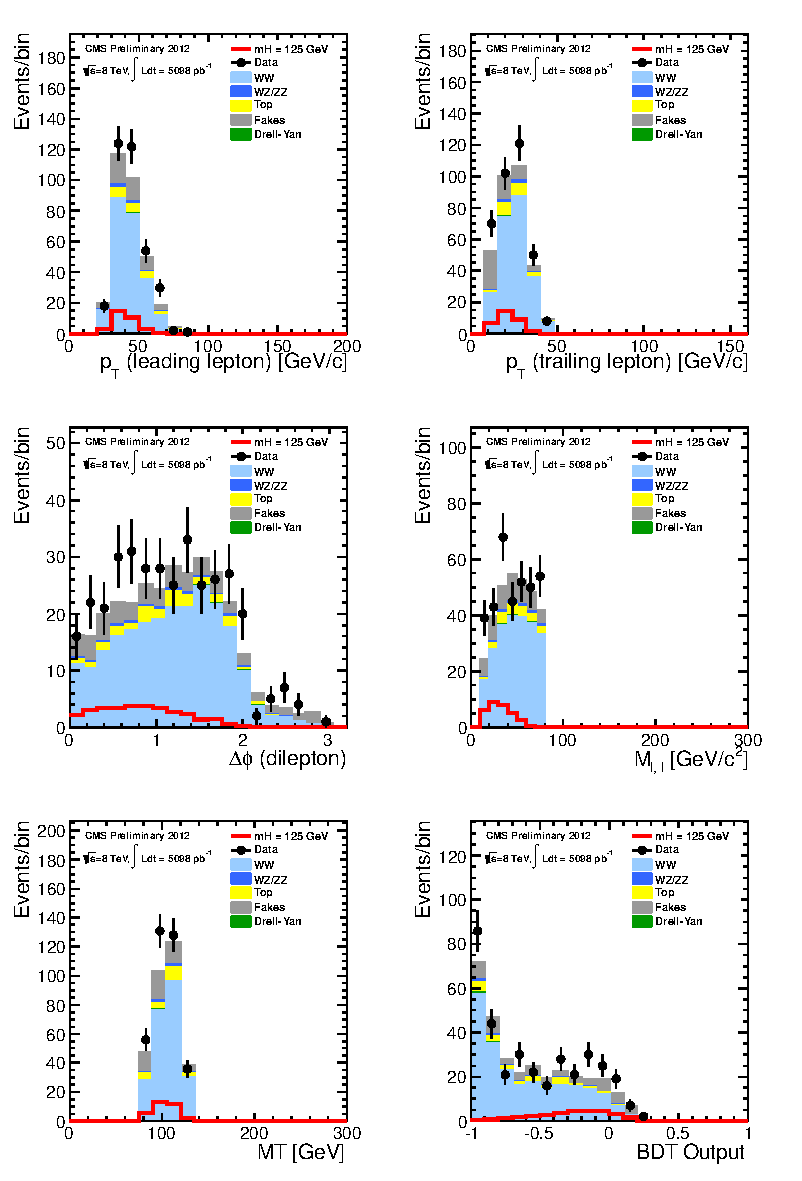
\includegraphics[width=1.0\textwidth]{figures/hww_analysis18_125_ALL_of_0j.pdf}
\caption{Kinematic distributions in the 0-jet bin in the opposite flavor final states for $m_{H}=125 ~\GeV$.}
\label{fig:hww_kinematics_125_0j}
\end{figure}
\begin{figure}[!htp]
\centering
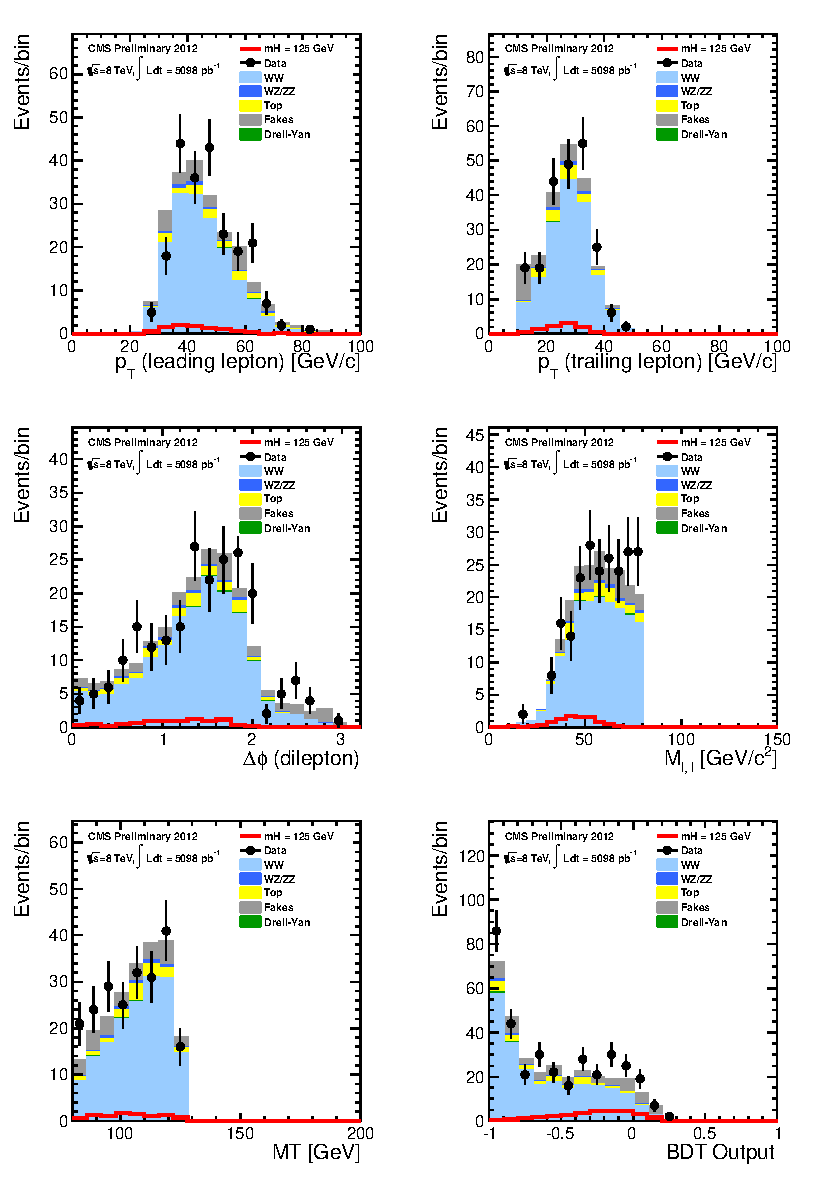
\includegraphics[width=1.0\textwidth]{figures/hww_bdtlo_analysis18_125_ALL_of_0j.pdf}
\caption{Kinematic distributions in the 0-jet bin in the opposite flavor final states for $m_{H}=125 ~\GeV$ (BDT$< -0.4$).}
\label{fig:hww_bdtlo_kinematics_125_0j}
\end{figure}
\begin{figure}[!htp]
\centering
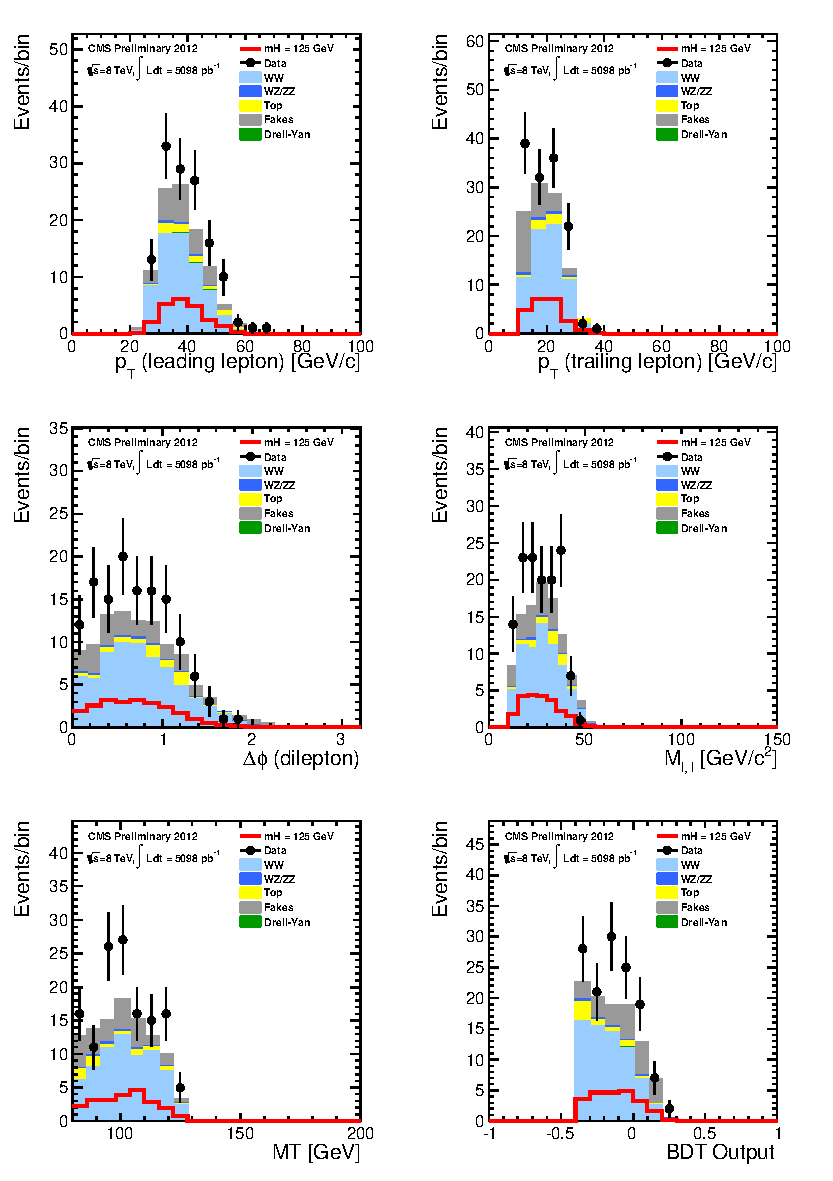
\includegraphics[width=1.0\textwidth]{figures/hww_bdthi_analysis18_125_ALL_of_0j.pdf}
\caption{Kinematic distributions in the 0-jet bin in the opposite flavor final states for $m_{H}=125 ~\GeV$ (BDT$> -0.4$).}
\label{fig:hww_bdthi_kinematics_125_0j}
\end{figure}
\begin{figure}[!htp]
\centering
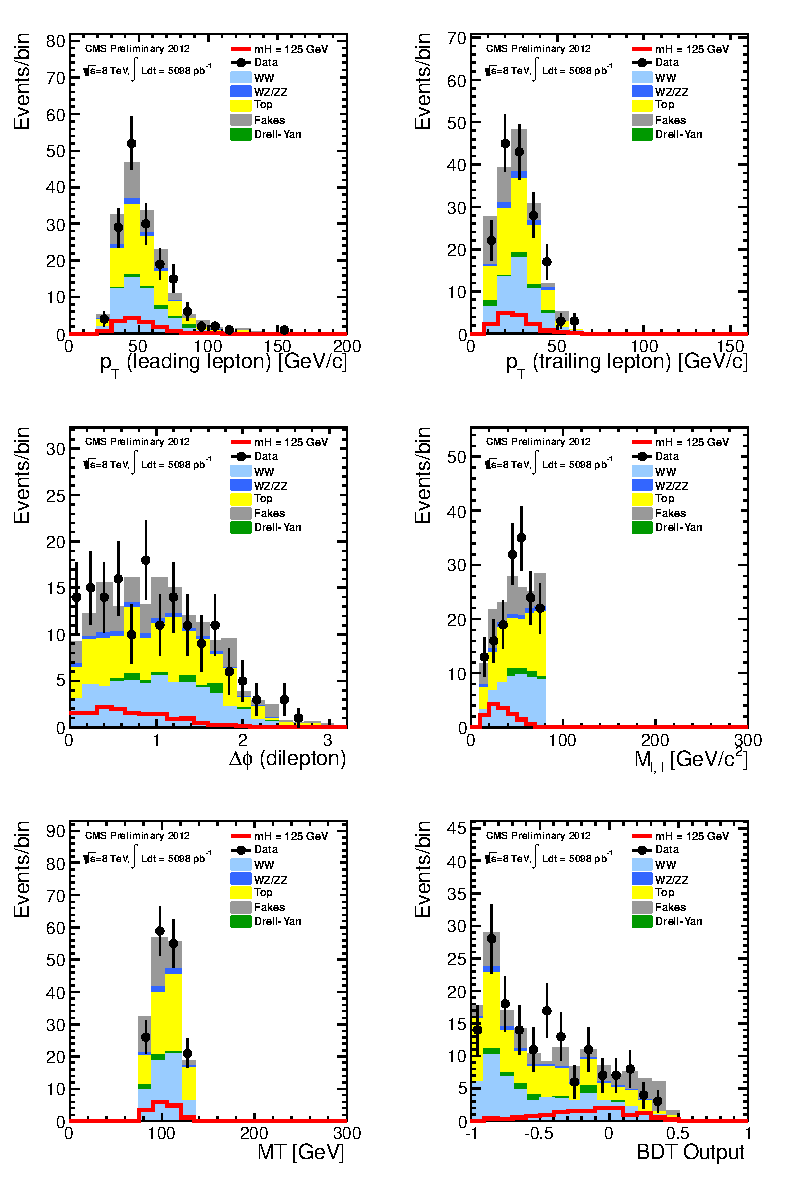
\includegraphics[width=1.0\textwidth]{figures/hww_analysis18_125_ALL_of_1j.pdf}
\caption{Kinematic distributions in the 1-jet bin in the opposite flavor final states for $m_{H}=125 ~\GeV$.}
\label{fig:hww_kinematics_125_1j}
\end{figure}
\begin{figure}[!htp]
\centering
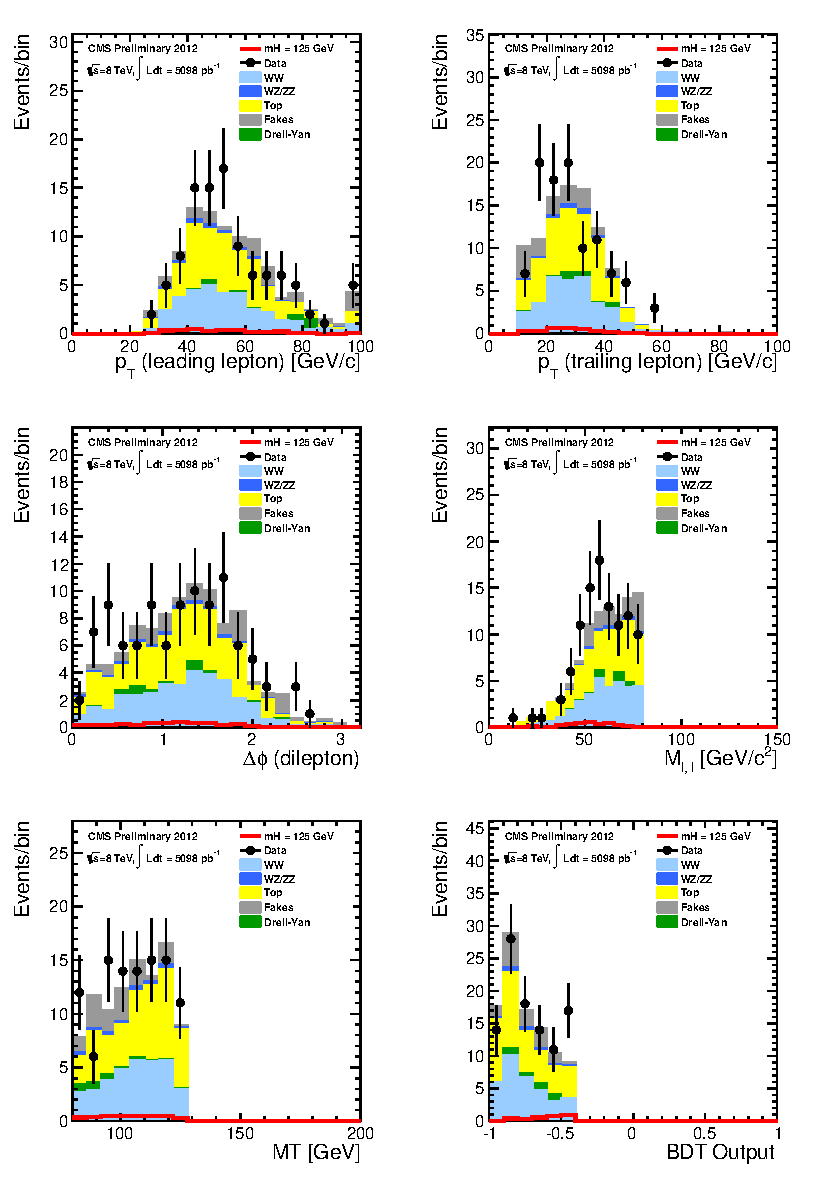
\includegraphics[width=1.0\textwidth]{figures/hww_bdtlo_analysis18_125_ALL_of_1j.pdf}
\caption{Kinematic distributions in the 1-jet bin in the opposite flavor final states for $m_{H}=125 ~\GeV$ (BDT$< -0.4$).}
\label{fig:hww_bdtlo_kinematics_125_1j}
\end{figure}
\begin{figure}[!htp]
\centering
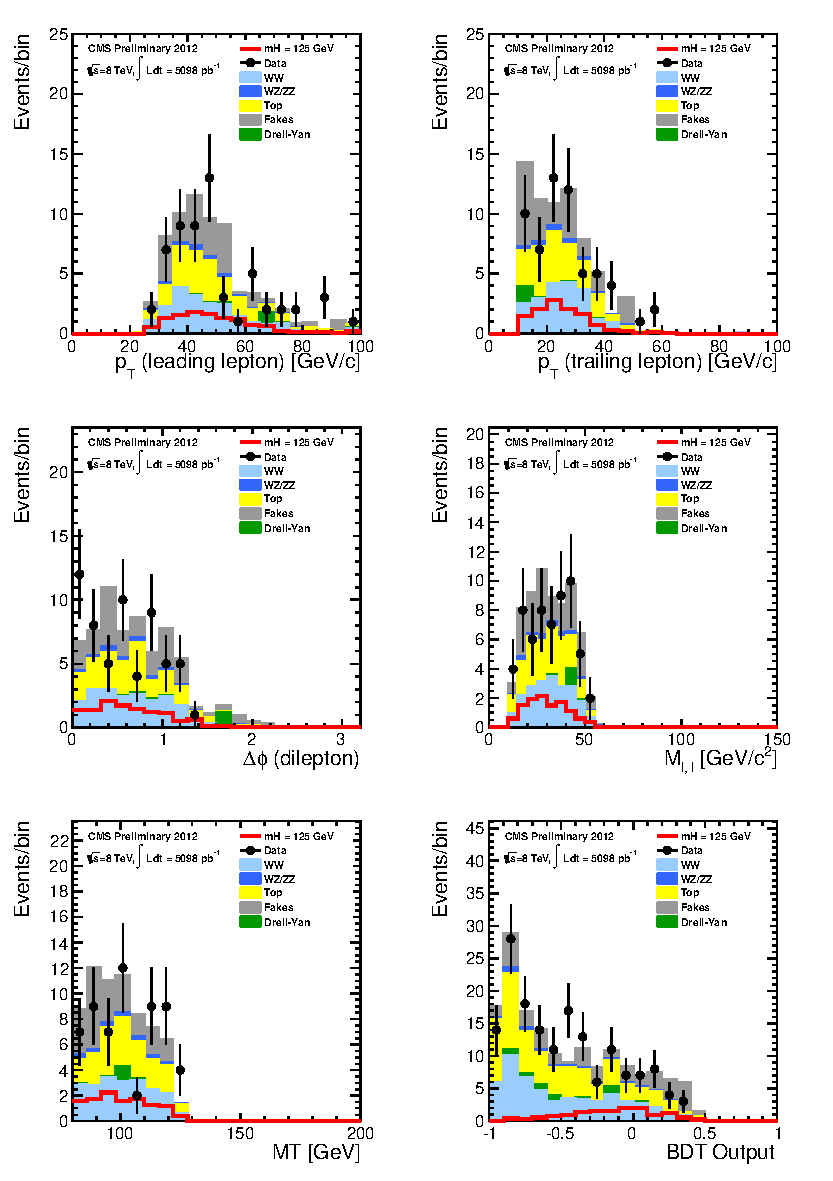
\includegraphics[width=1.0\textwidth]{figures/hww_bdthi_analysis18_125_ALL_of_1j.pdf}
\caption{Kinematic distributions in the 1-jet bin in the opposite flavor final states for $m_{H}=125 ~\GeV$ (BDT$> -0.4$).}
\label{fig:hww_bdthi_kinematics_125_1j}
\end{figure}
%%%%%%%%%%%%%%

\clearpage
%%%%%%%%%%%%%%
\begin{figure}[!htp]
\centering
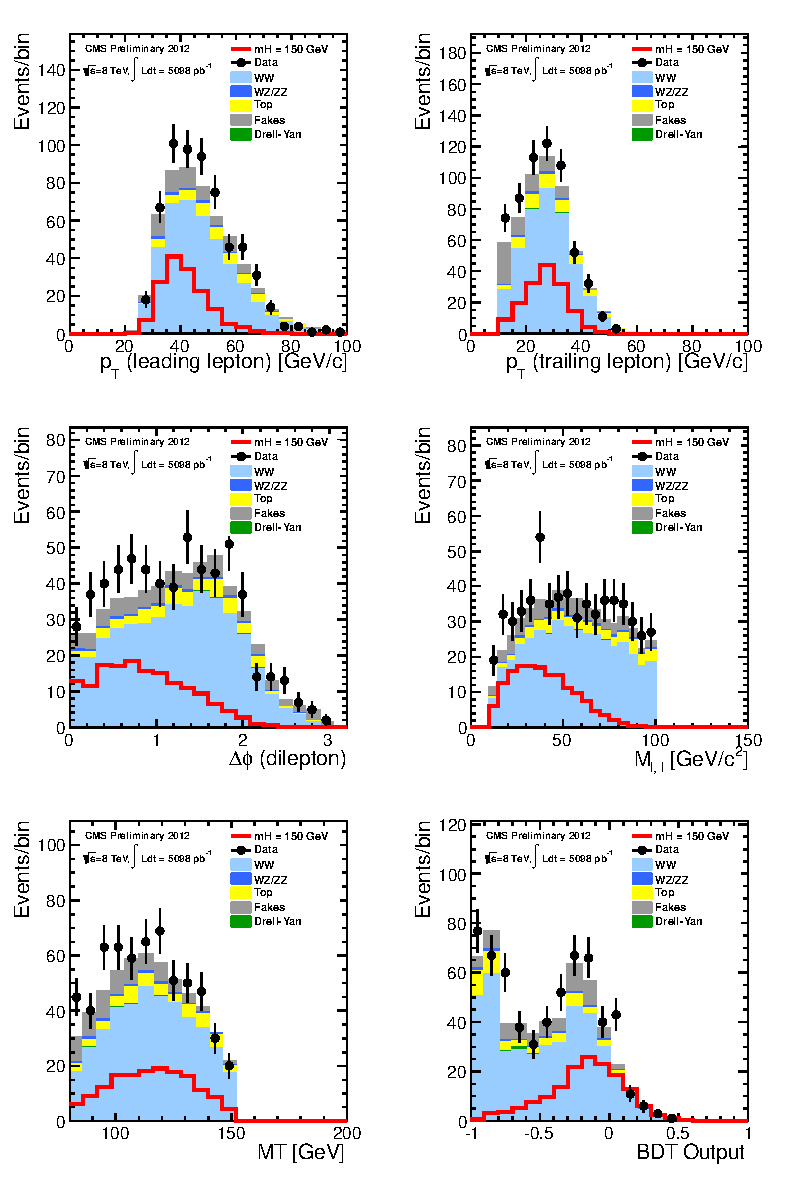
\includegraphics[width=1.0\textwidth]{figures/hww_analysis18_150_ALL_of_0j.pdf}
\caption{Kinematic distributions in the 0-jet bin in the opposite flavor final states for $m_{H}=150 ~\GeV$.}
\label{fig:hww_kinematics_150_0j}
\end{figure}
\begin{figure}[!htp]
\centering
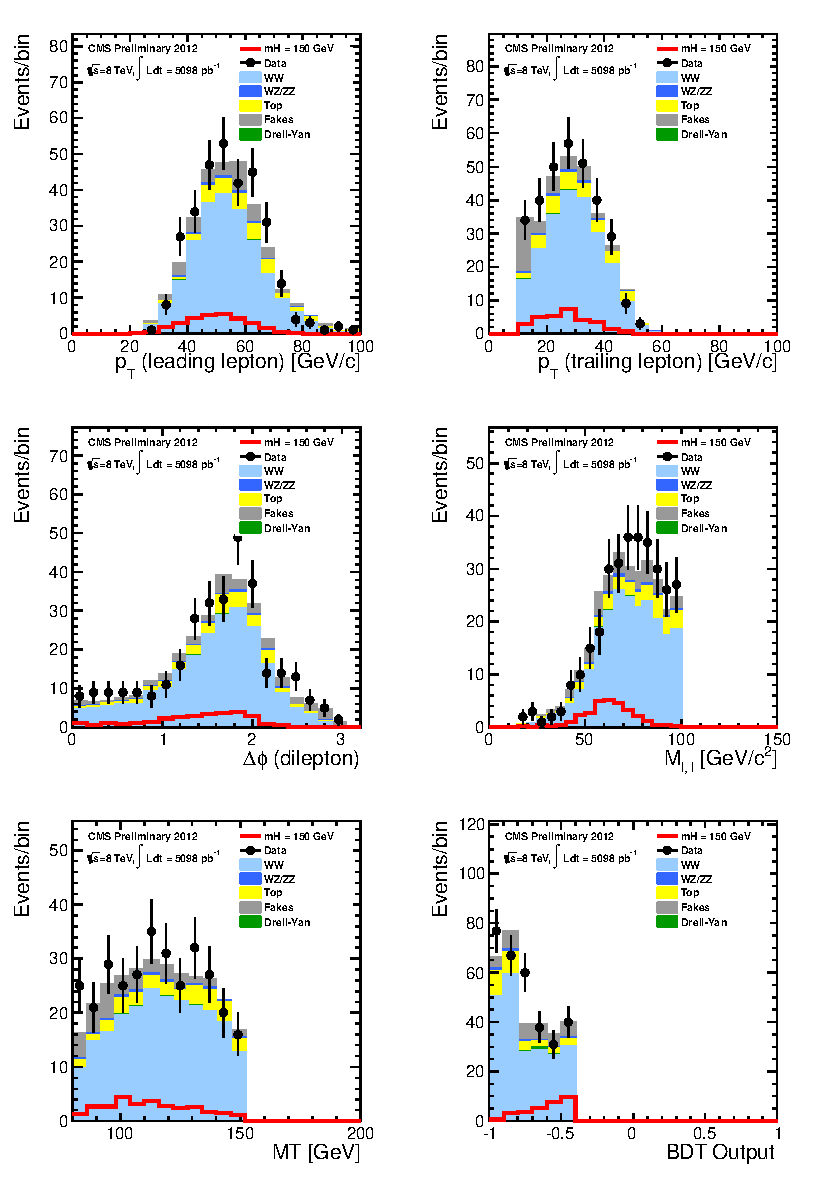
\includegraphics[width=1.0\textwidth]{figures/hww_bdtlo_analysis18_150_ALL_of_0j.pdf}
\caption{Kinematic distributions in the 0-jet bin in the opposite flavor final states for $m_{H}=150 ~\GeV$ (BDT$< -0.4$).}
\label{fig:hww_bdtlo_kinematics_150_0j}
\end{figure}
\begin{figure}[!htp]
\centering
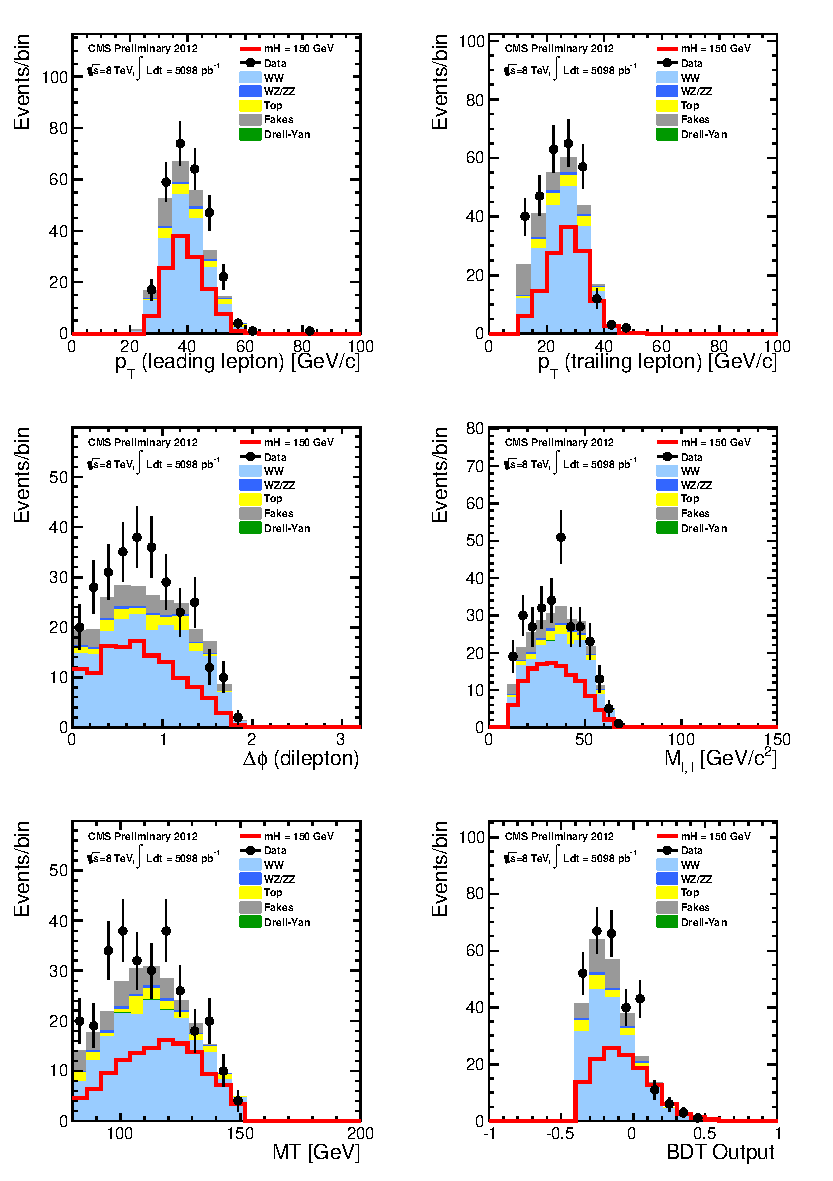
\includegraphics[width=1.0\textwidth]{figures/hww_bdthi_analysis18_150_ALL_of_0j.pdf}
\caption{Kinematic distributions in the 0-jet bin in the opposite flavor final states for $m_{H}=150 ~\GeV$ (BDT$> -0.4$).}
\label{fig:hww_bdthi_kinematics_150_0j}
\end{figure}
\begin{figure}[!htp]
\centering
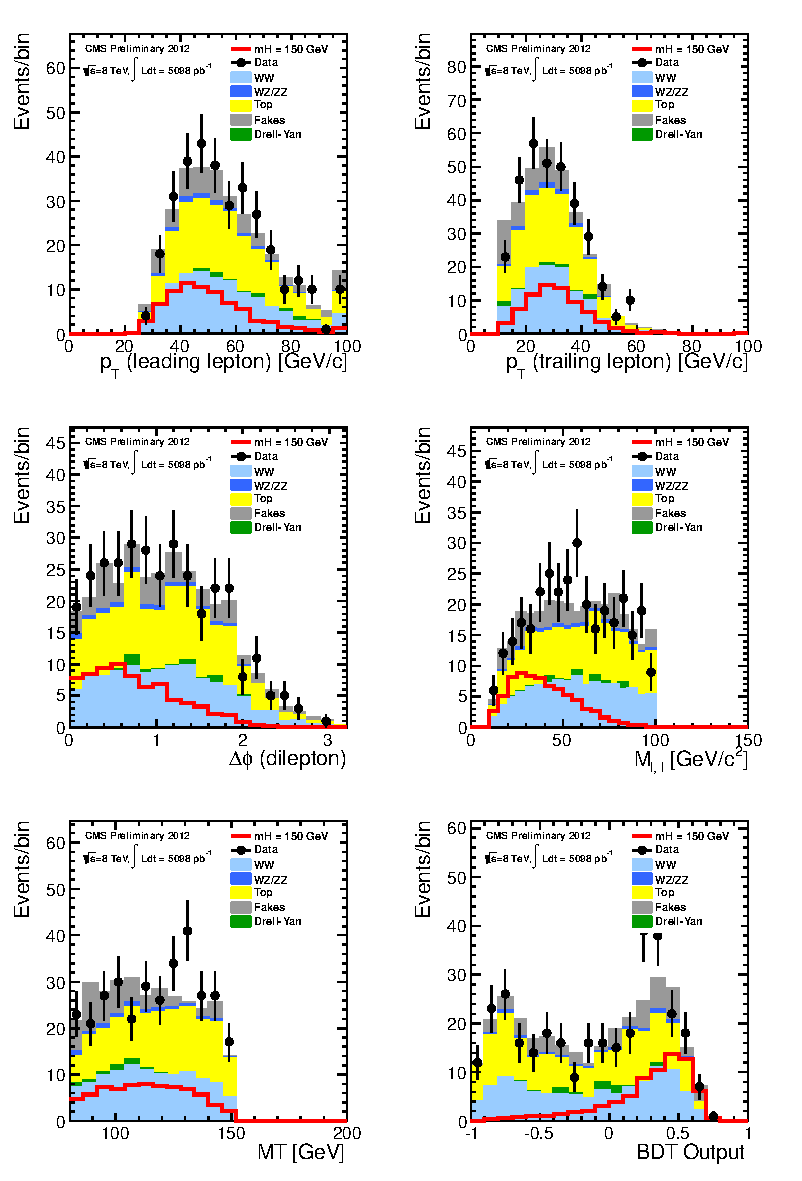
\includegraphics[width=1.0\textwidth]{figures/hww_analysis18_150_ALL_of_1j.pdf}
\caption{Kinematic distributions in the 1-jet bin in the opposite flavor final states for $m_{H}=150 ~\GeV$.}
\label{fig:hww_kinematics_150_1j}
\end{figure}
\begin{figure}[!htp]
\centering
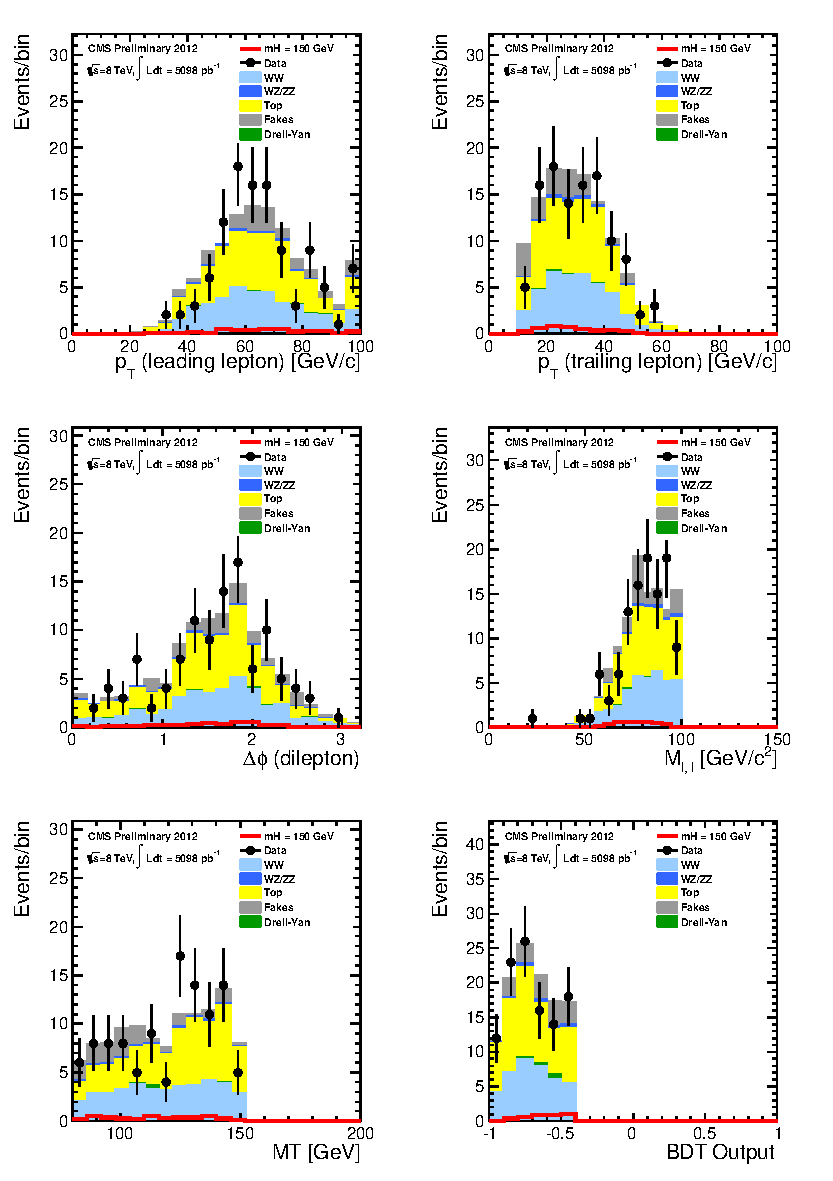
\includegraphics[width=1.0\textwidth]{figures/hww_bdtlo_analysis18_150_ALL_of_1j.pdf}
\caption{Kinematic distributions in the 1-jet bin in the opposite flavor final states for $m_{H}=150 ~\GeV$ (BDT$< -0.4$).}
\label{fig:hww_bdtlo_kinematics_150_1j}
\end{figure}
\begin{figure}[!htp]
\centering
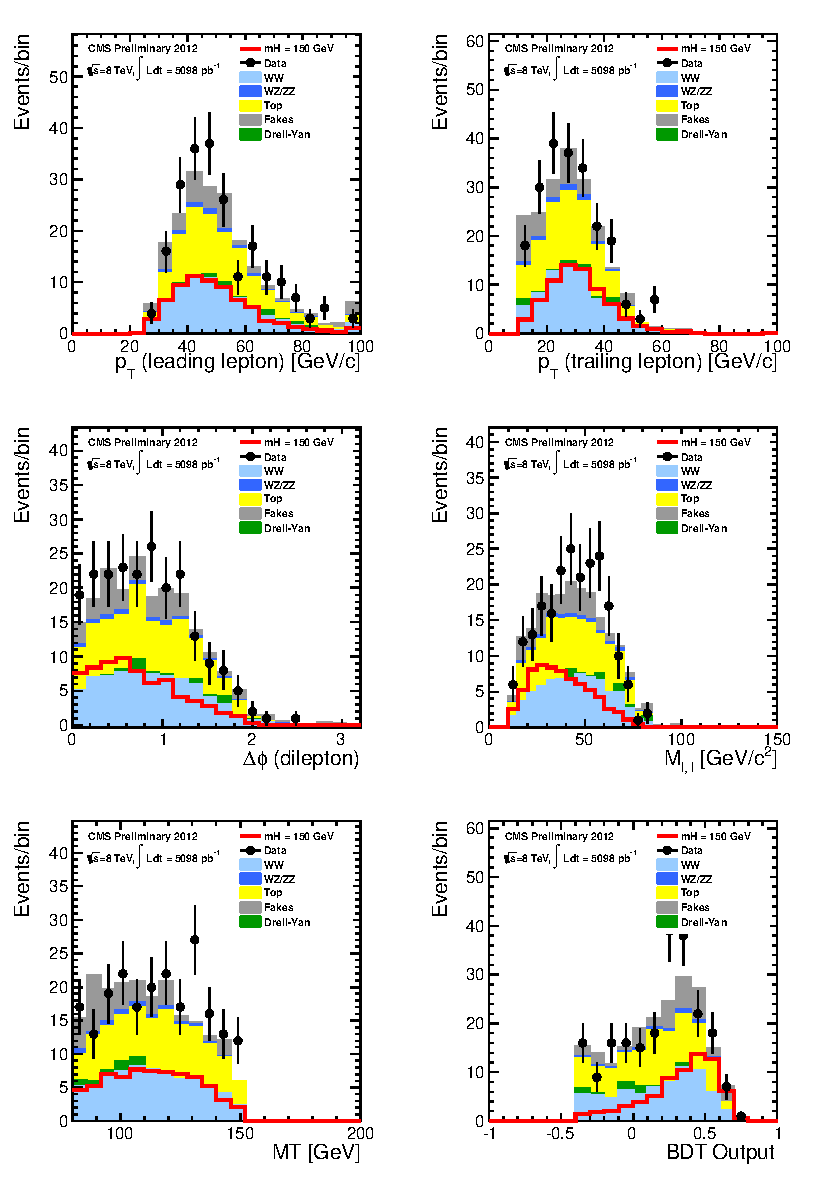
\includegraphics[width=1.0\textwidth]{figures/hww_bdthi_analysis18_150_ALL_of_1j.pdf}
\caption{Kinematic distributions in the 1-jet bin in the opposite flavor final states for $m_{H}=150 ~\GeV$ (BDT$> -0.4$).}
\label{fig:hww_bdthi_kinematics_150_1j}
\end{figure}
%%%%%%%%%%%%%%

\clearpage
%%%%%%%%%%%%%%
\begin{figure}[!htp]
\centering
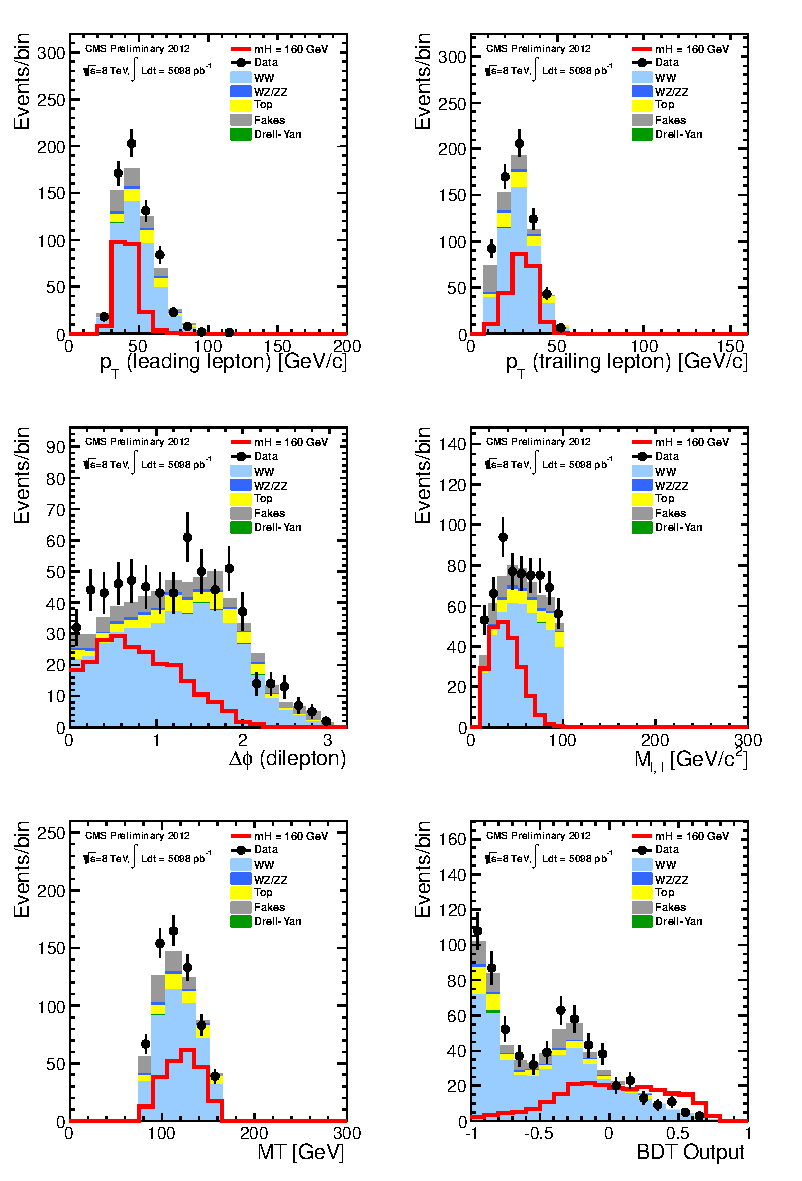
\includegraphics[width=1.0\textwidth]{figures/hww_analysis18_160_ALL_of_0j.pdf}
\caption{Kinematic distributions in the 0-jet bin in the opposite flavor final states for $m_{H}=160 ~\GeV$.}
\label{fig:hww_kinematics_160_0j}
\end{figure}
\begin{figure}[!htp]
\centering
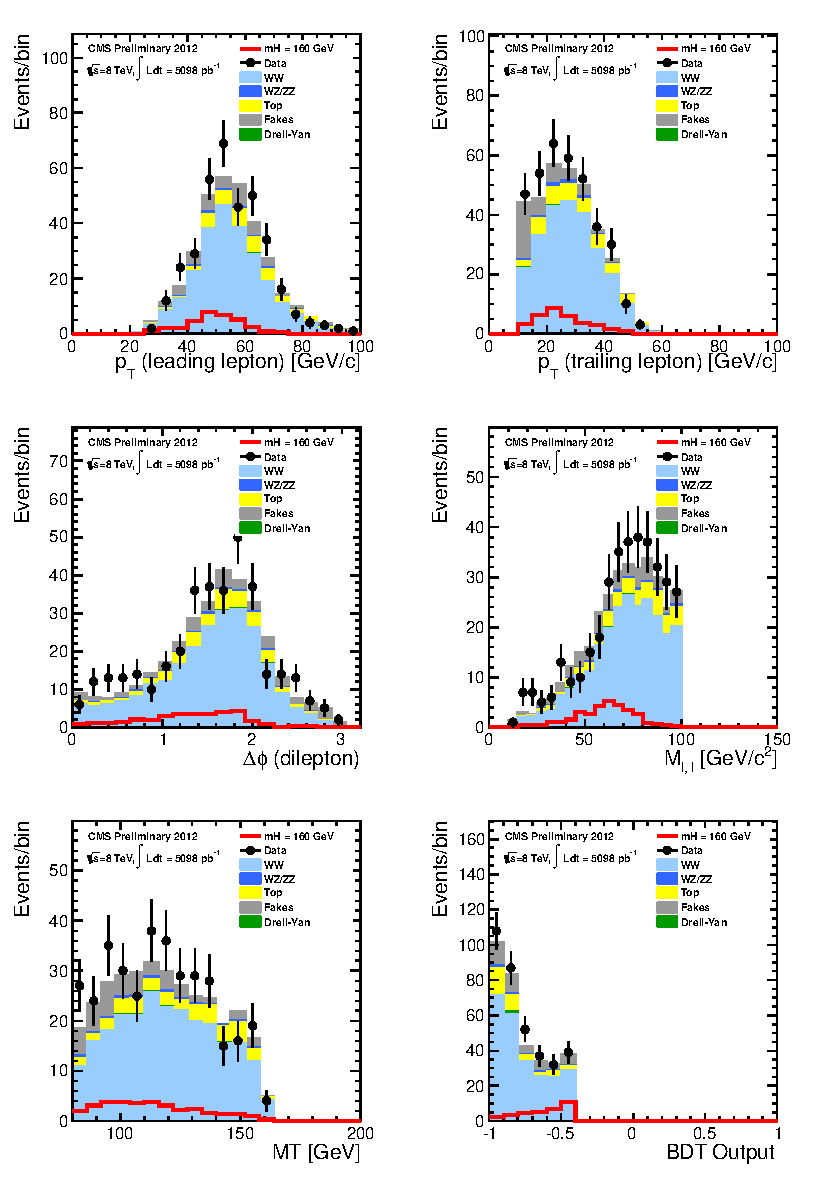
\includegraphics[width=1.0\textwidth]{figures/hww_bdtlo_analysis18_160_ALL_of_0j.pdf}
\caption{Kinematic distributions in the 0-jet bin in the opposite flavor final states for $m_{H}=160 ~\GeV$ (BDT$< -0.4$).}
\label{fig:hww_bdtlo_kinematics_160_0j}
\end{figure}
\begin{figure}[!htp]
\centering
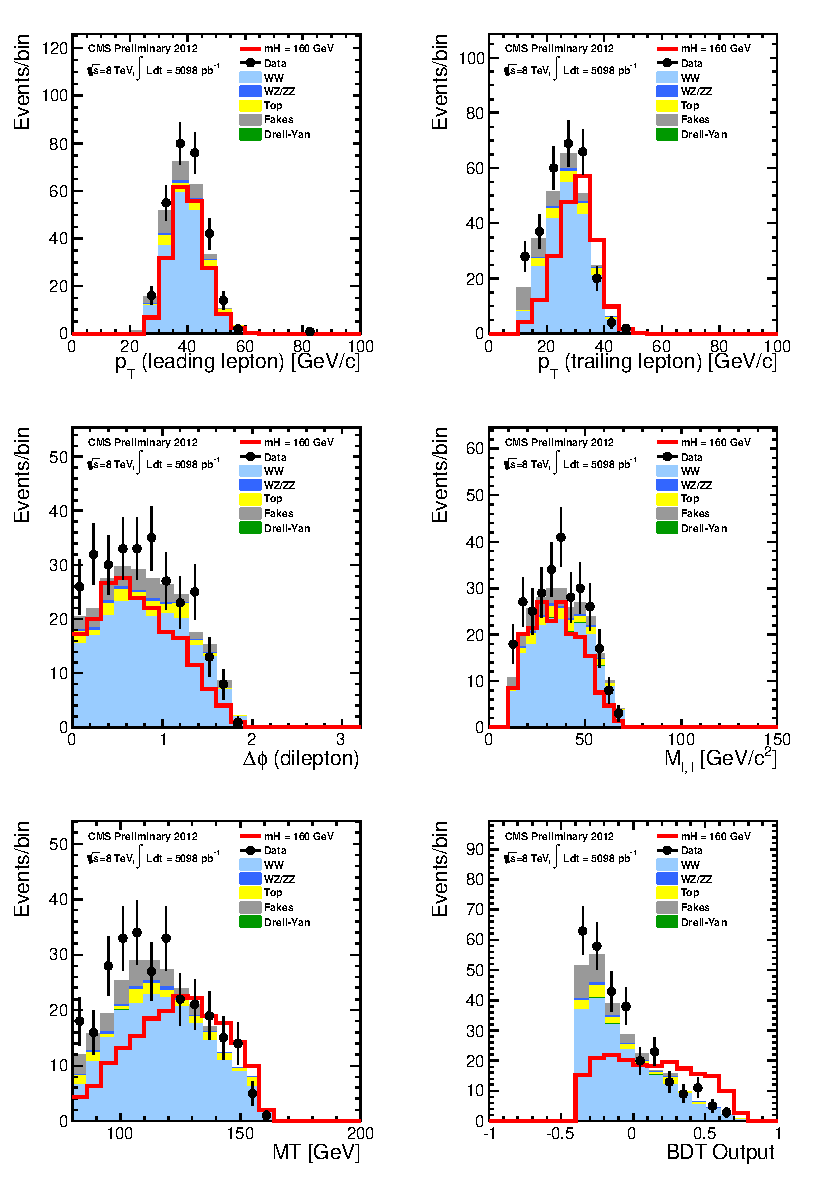
\includegraphics[width=1.0\textwidth]{figures/hww_bdthi_analysis18_160_ALL_of_0j.pdf}
\caption{Kinematic distributions in the 0-jet bin in the opposite flavor final states for $m_{H}=160 ~\GeV$ (BDT$> -0.4$).}
\label{fig:hww_bdthi_kinematics_160_0j}
\end{figure}
\begin{figure}[!htp]
\centering
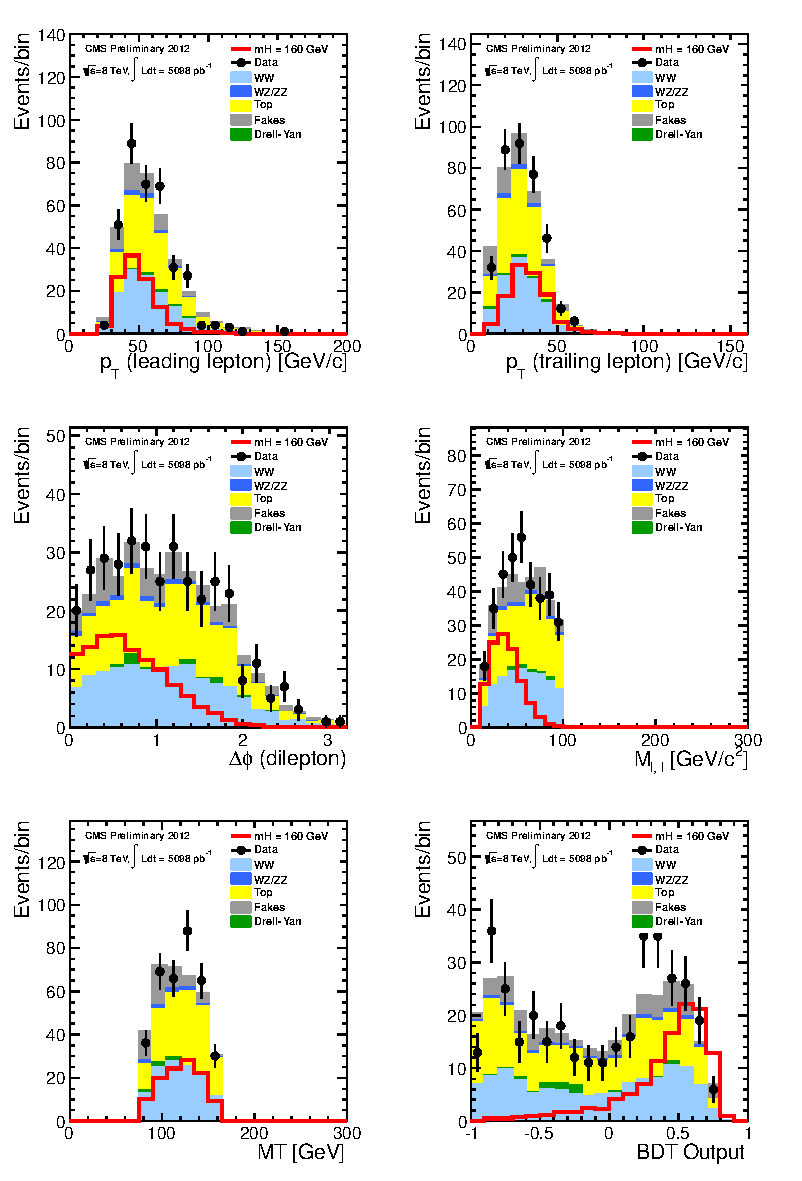
\includegraphics[width=1.0\textwidth]{figures/hww_analysis18_160_ALL_of_1j.pdf}
\caption{Kinematic distributions in the 1-jet bin in the opposite flavor final states for $m_{H}=160 ~\GeV$.}
\label{fig:hww_kinematics_160_1j}
\end{figure}
\begin{figure}[!htp]
\centering
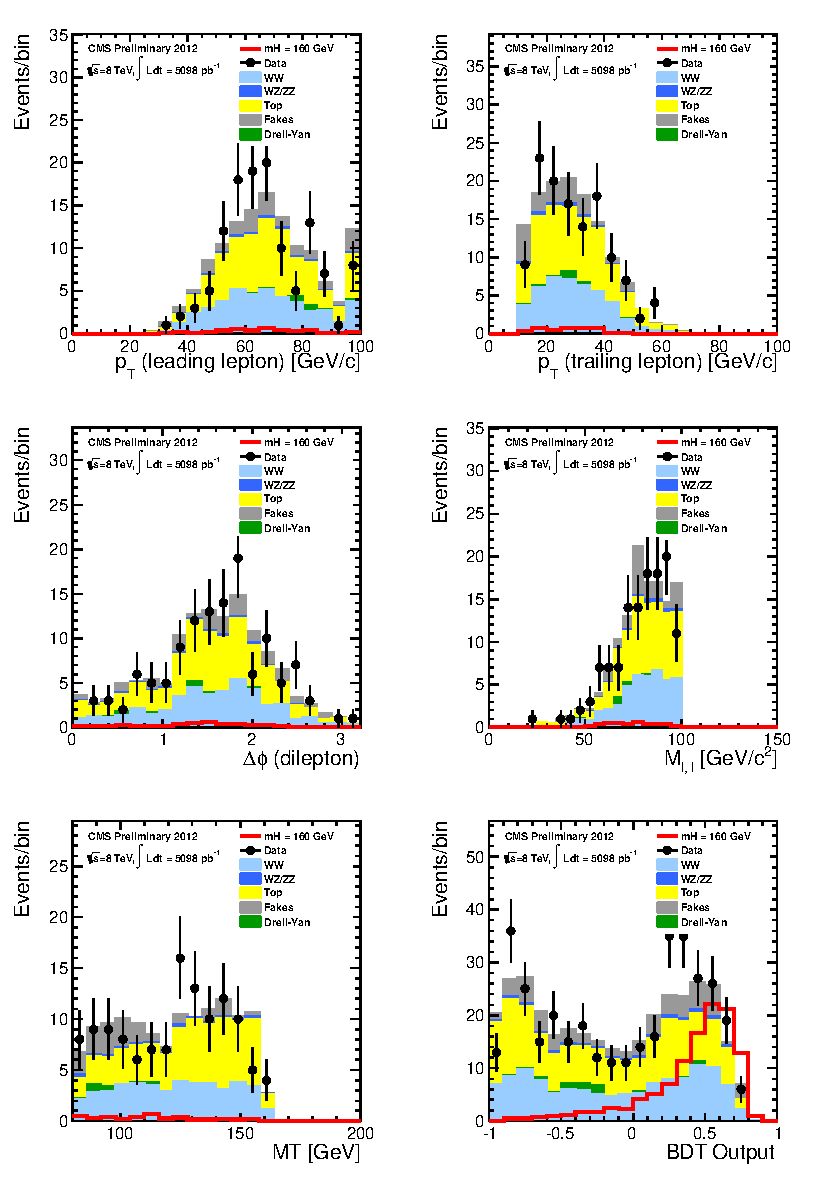
\includegraphics[width=1.0\textwidth]{figures/hww_bdtlo_analysis18_160_ALL_of_1j.pdf}
\caption{Kinematic distributions in the 1-jet bin in the opposite flavor final states for $m_{H}=160 ~\GeV$ (BDT$< -0.4$).}
\label{fig:hww_bdtlo_kinematics_160_1j}
\end{figure}
\begin{figure}[!htp]
\centering
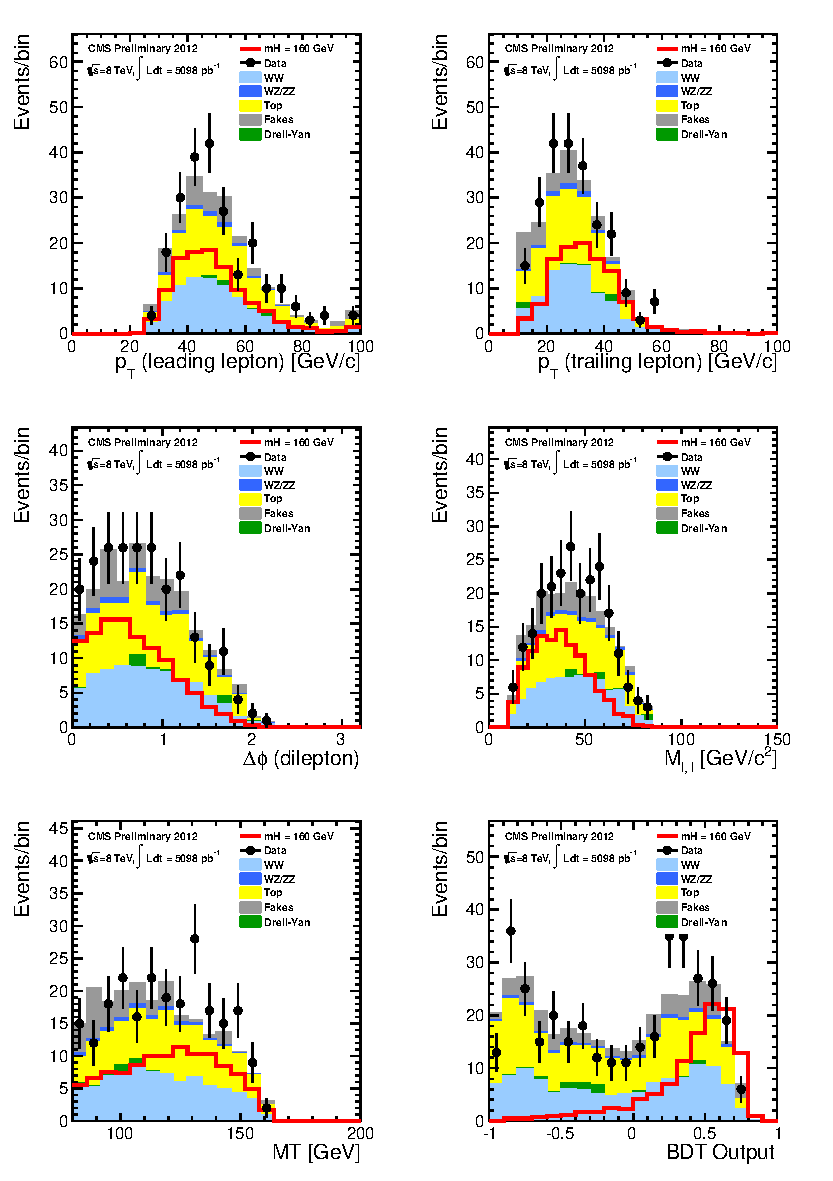
\includegraphics[width=1.0\textwidth]{figures/hww_bdthi_analysis18_160_ALL_of_1j.pdf}
\caption{Kinematic distributions in the 1-jet bin in the opposite flavor final states for $m_{H}=160 ~\GeV$ (BDT$> -0.4$).}
\label{fig:hww_bdthi_kinematics_160_1j}
\end{figure}
%%%%%%%%%%%%%%

\clearpage
%%%%%%%%%%%%%%
\begin{figure}[!htp]
\centering
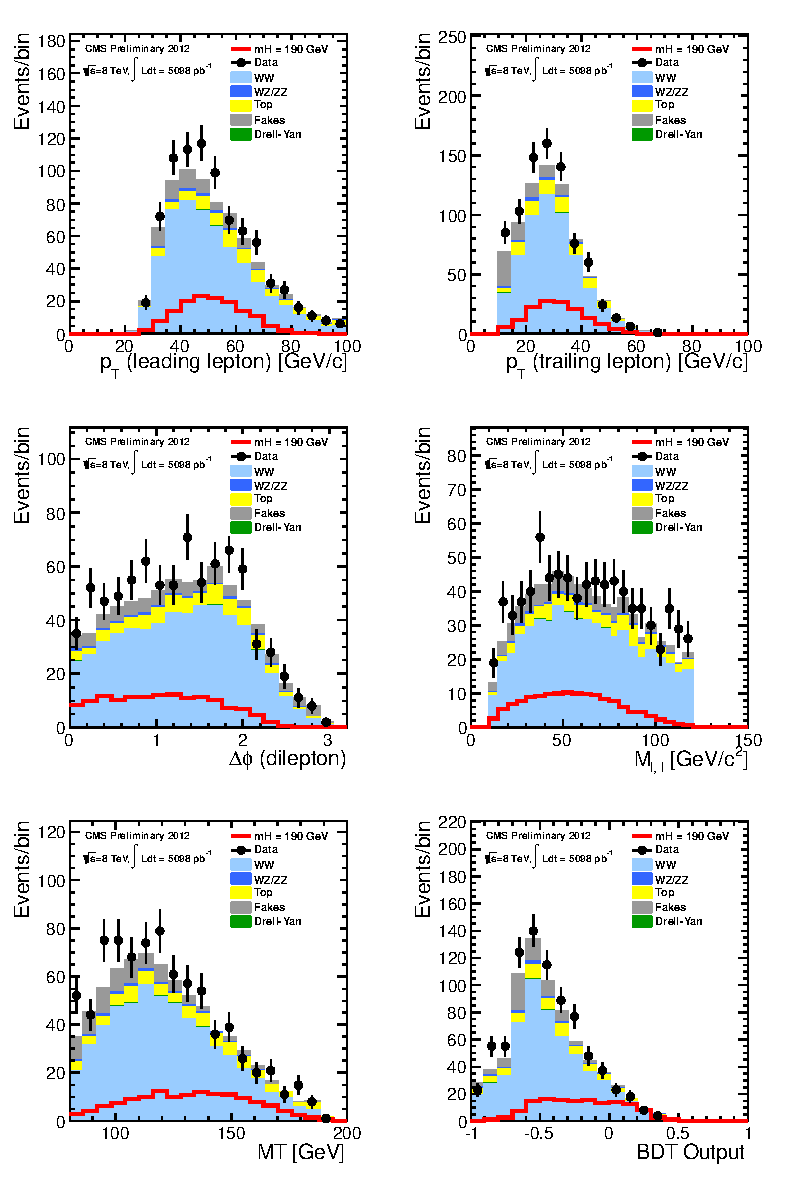
\includegraphics[width=1.0\textwidth]{figures/hww_analysis18_190_ALL_of_0j.pdf}
\caption{Kinematic distributions in the 0-jet bin in the opposite flavor final states for $m_{H}=190 ~\GeV$.}
\label{fig:hww_kinematics_190_0j}
\end{figure}
\begin{figure}[!htp]
\centering
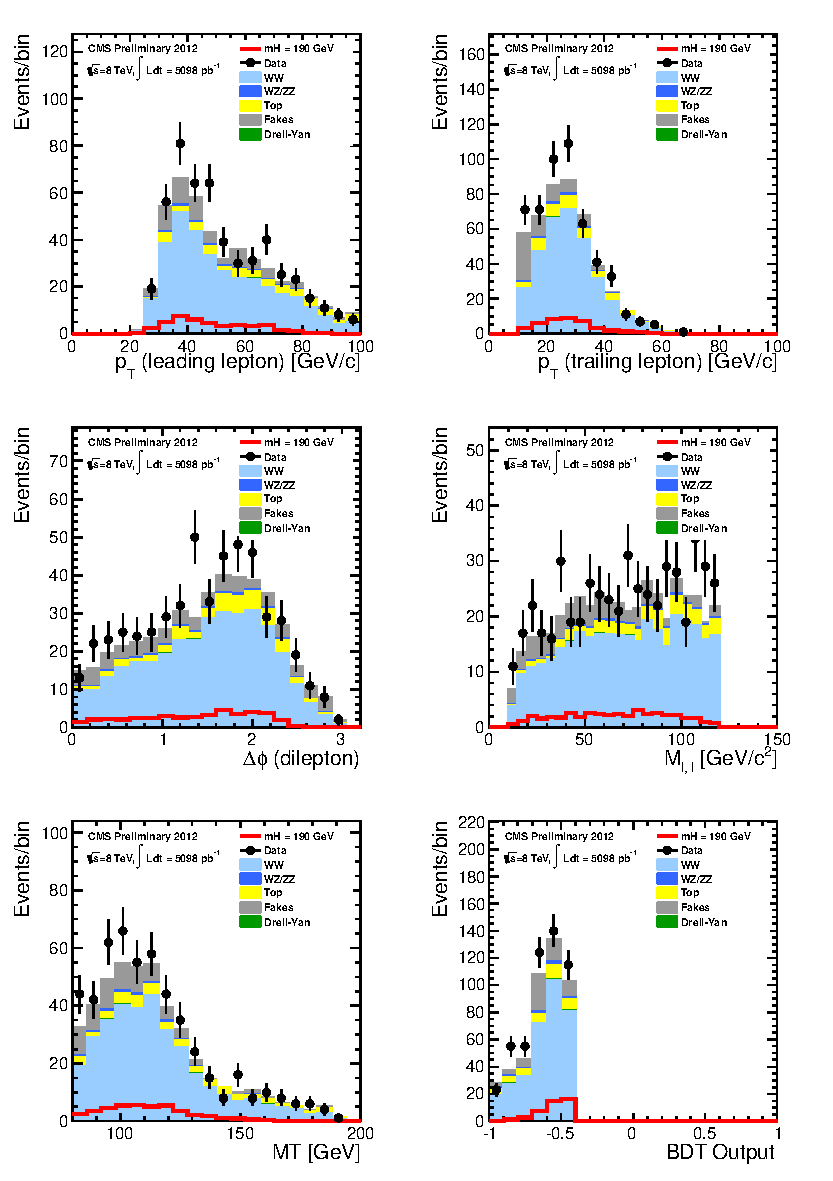
\includegraphics[width=1.0\textwidth]{figures/hww_bdtlo_analysis18_190_ALL_of_0j.pdf}
\caption{Kinematic distributions in the 0-jet bin in the opposite flavor final states for $m_{H}=190 ~\GeV$ (BDT$< -0.4$).}
\label{fig:hww_bdtlo_kinematics_190_0j}
\end{figure}
\begin{figure}[!htp]
\centering
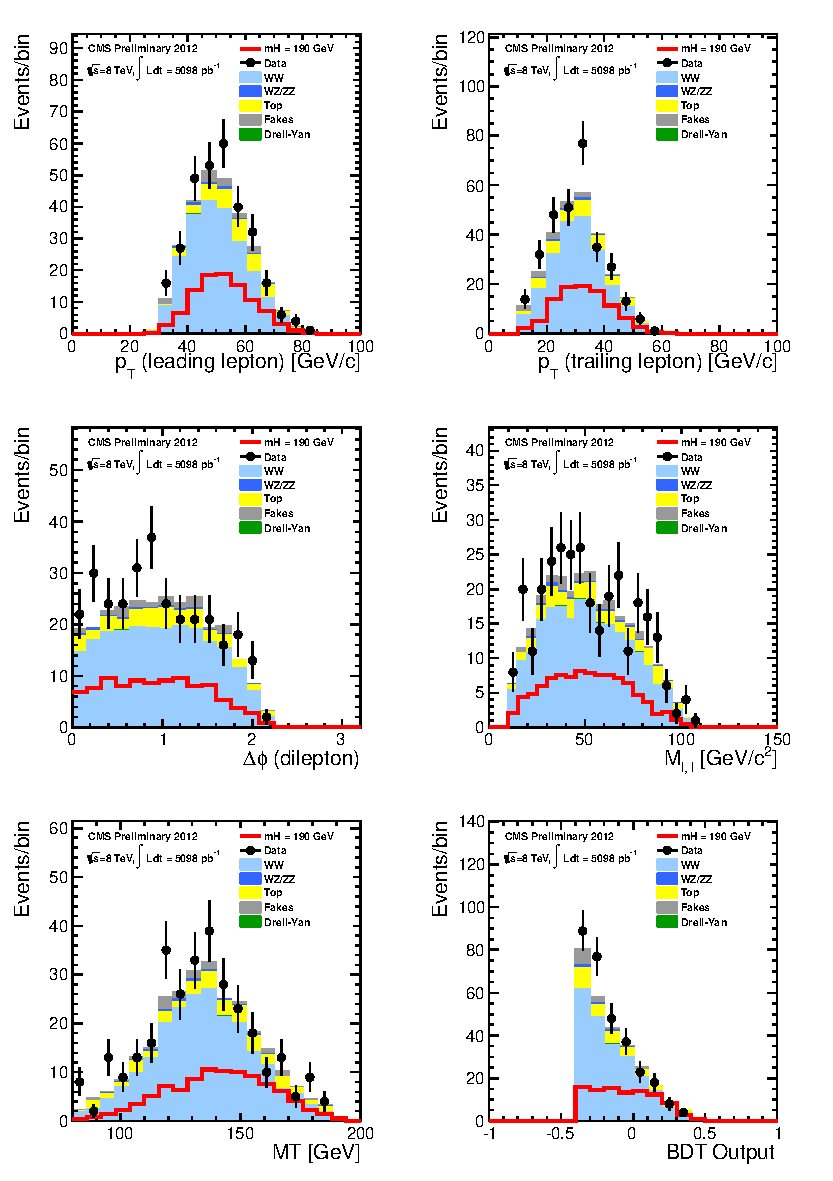
\includegraphics[width=1.0\textwidth]{figures/hww_bdthi_analysis18_190_ALL_of_0j.pdf}
\caption{Kinematic distributions in the 0-jet bin in the opposite flavor final states for $m_{H}=190 ~\GeV$ (BDT$> -0.4$).}
\label{fig:hww_bdthi_kinematics_190_0j}
\end{figure}
\begin{figure}[!htp]
\centering
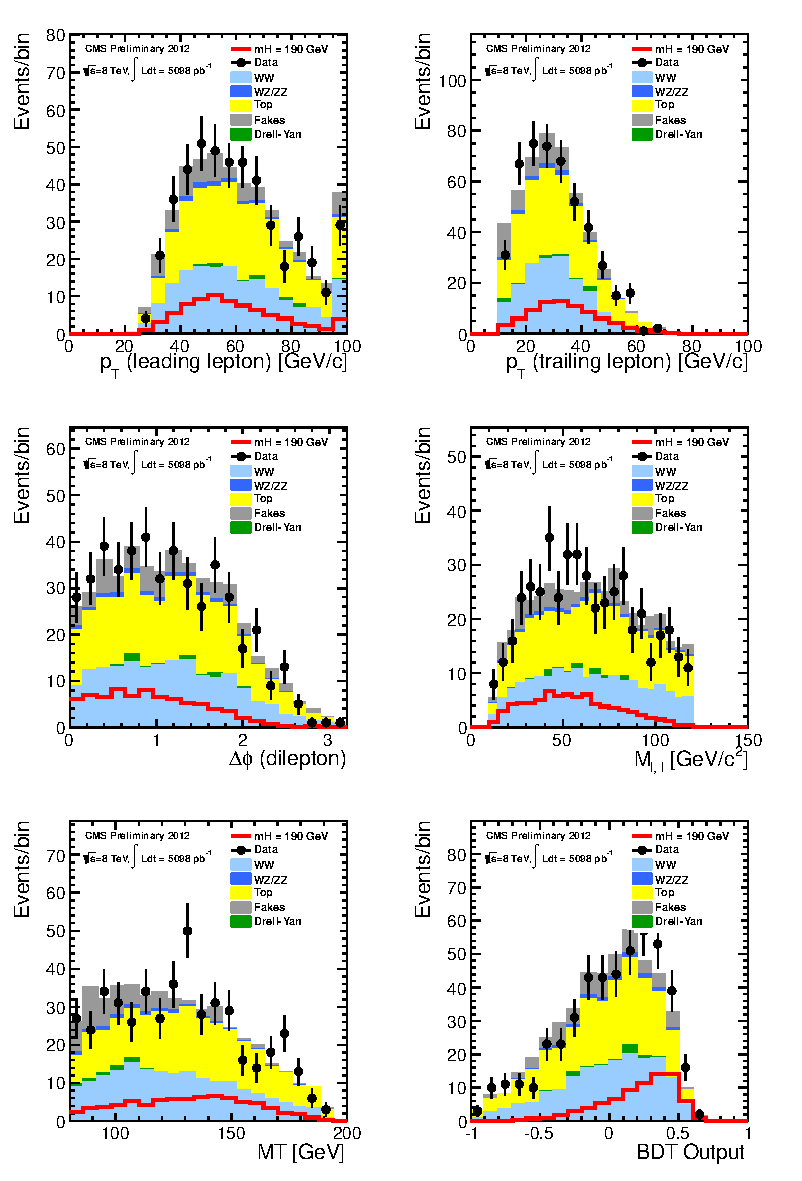
\includegraphics[width=1.0\textwidth]{figures/hww_analysis18_190_ALL_of_1j.pdf}
\caption{Kinematic distributions in the 1-jet bin in the opposite flavor final states for $m_{H}=190 ~\GeV$.}
\label{fig:hww_kinematics_190_1j}
\end{figure}
\begin{figure}[!htp]
\centering
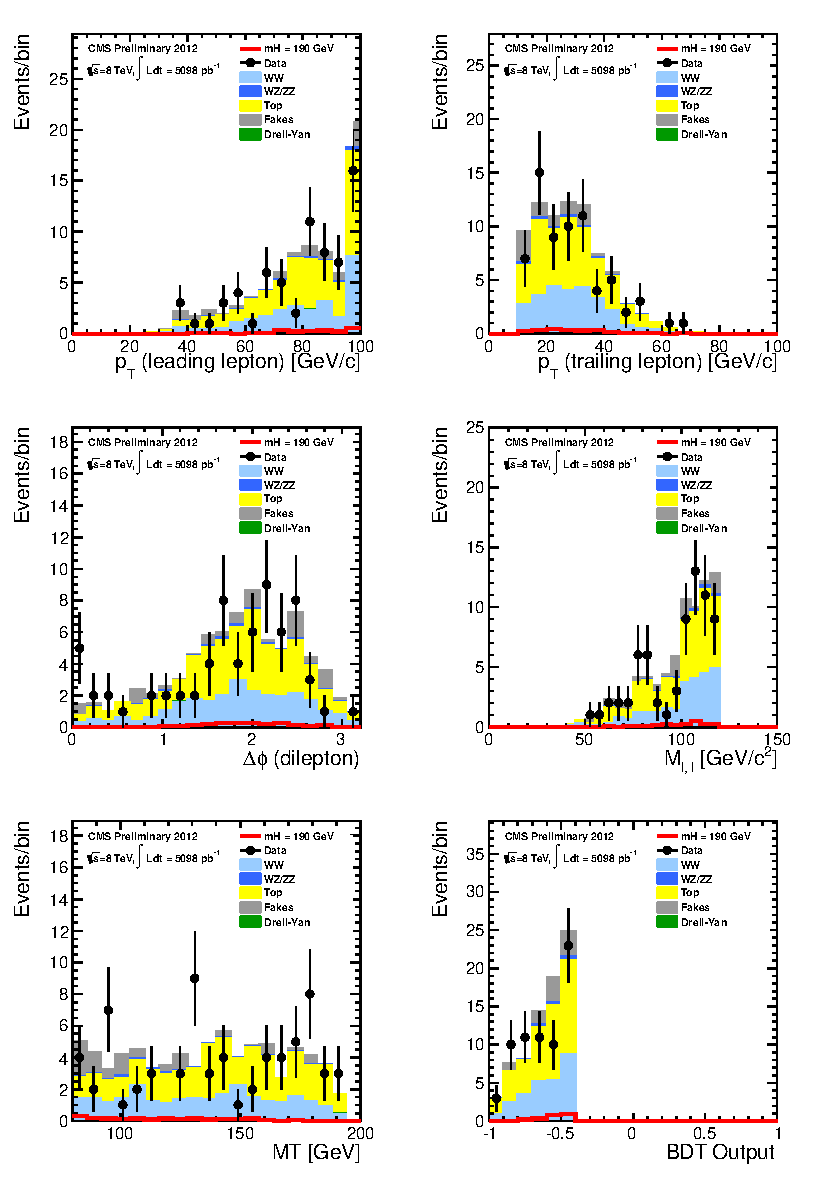
\includegraphics[width=1.0\textwidth]{figures/hww_bdtlo_analysis18_190_ALL_of_1j.pdf}
\caption{Kinematic distributions in the 1-jet bin in the opposite flavor final states for $m_{H}=190 ~\GeV$ (BDT$< -0.4$).}
\label{fig:hww_bdtlo_kinematics_190_1j}
\end{figure}
\begin{figure}[!htp]
\centering
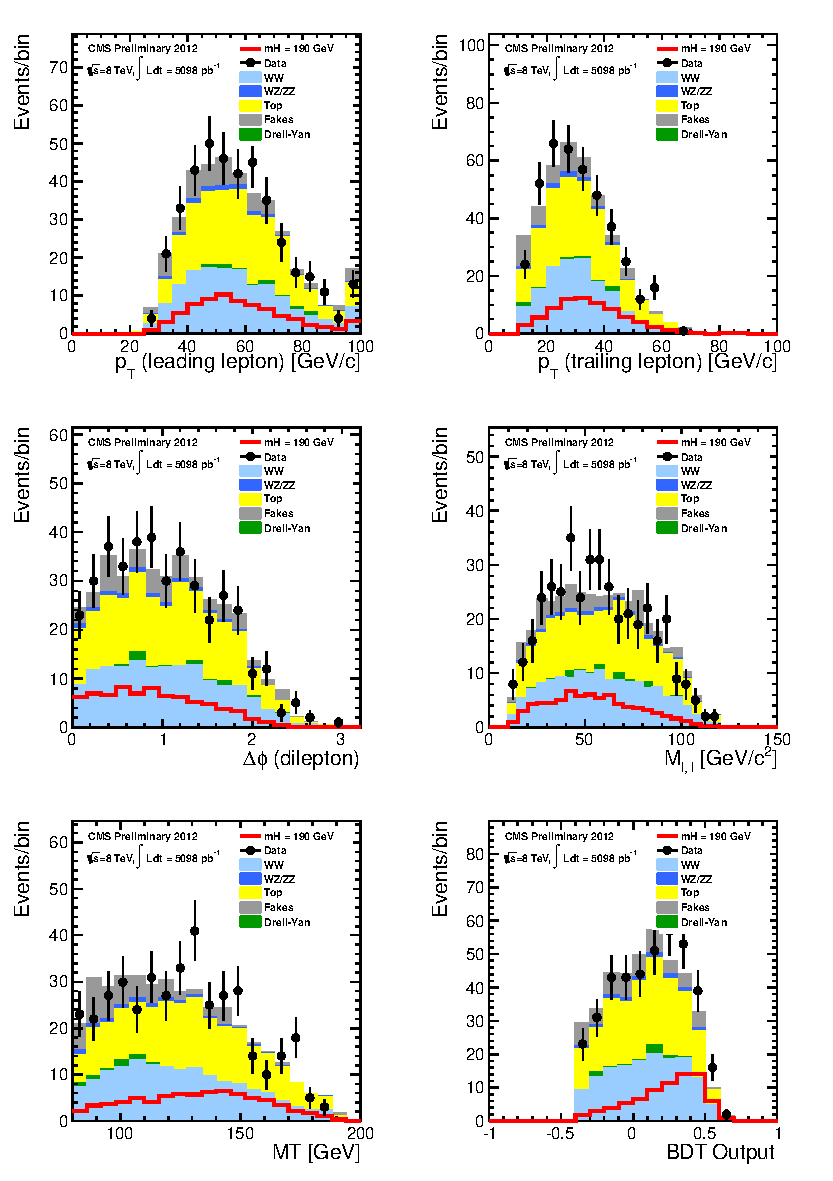
\includegraphics[width=1.0\textwidth]{figures/hww_bdthi_analysis18_190_ALL_of_1j.pdf}
\caption{Kinematic distributions in the 1-jet bin in the opposite flavor final states for $m_{H}=190 ~\GeV$ (BDT$> -0.4$).}
\label{fig:hww_bdthi_kinematics_190_1j}
\end{figure}
%%%%%%%%%%%%%%

\clearpage
%%%%%%%%%%%%%%
\begin{figure}[!htp]
\centering
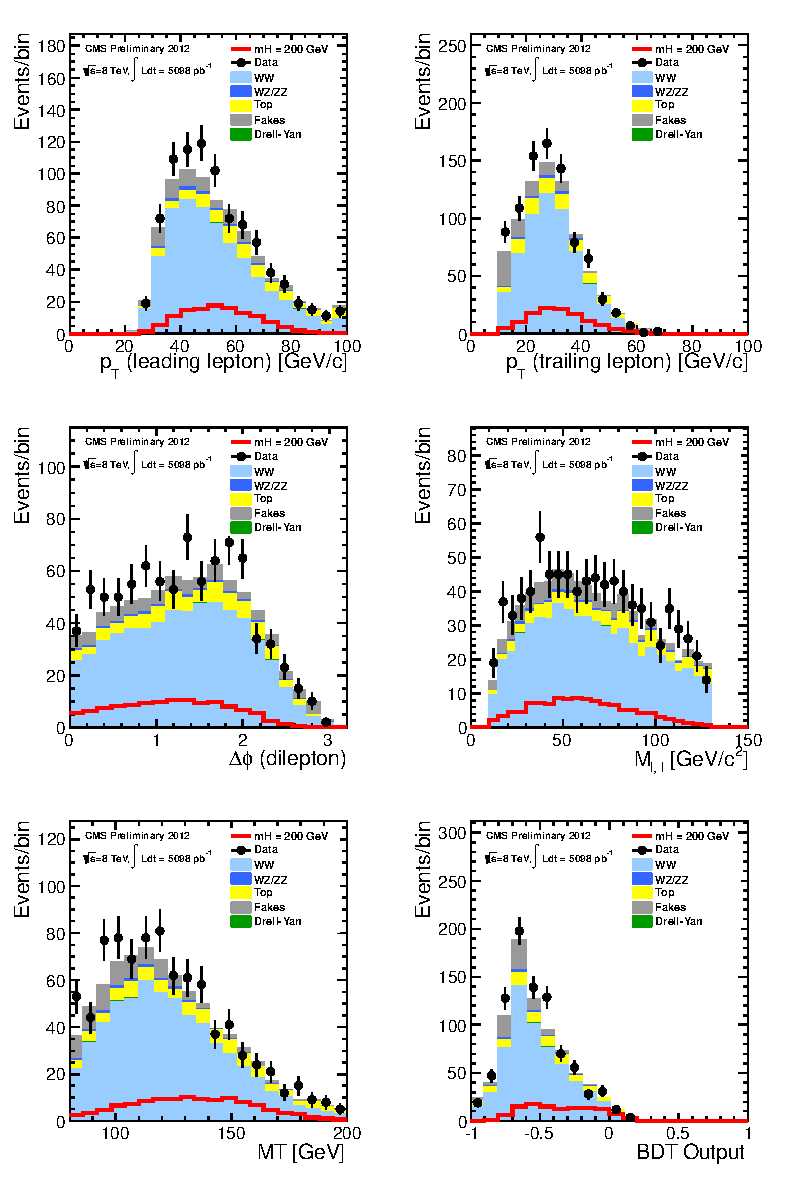
\includegraphics[width=1.0\textwidth]{figures/hww_analysis18_200_ALL_of_0j.pdf}
\caption{Kinematic distributions in the 0-jet bin in the opposite flavor final states for $m_{H}=200 ~\GeV$.}
\label{fig:hww_kinematics_200_0j}
\end{figure}
\begin{figure}[!htp]
\centering
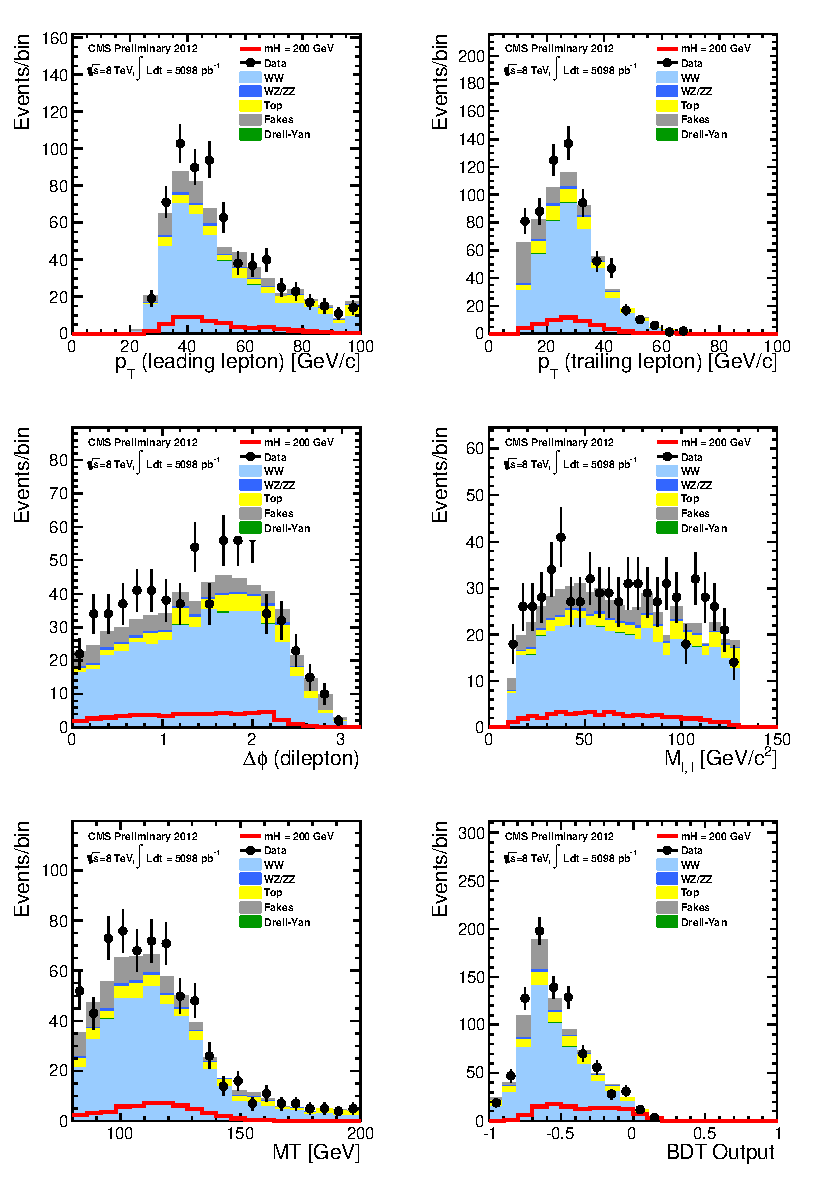
\includegraphics[width=1.0\textwidth]{figures/hww_bdtlo_analysis18_200_ALL_of_0j.pdf}
\caption{Kinematic distributions in the 0-jet bin in the opposite flavor final states for $m_{H}=200 ~\GeV$ (BDT$< -0.4$).}
\label{fig:hww_bdtlo_kinematics_200_0j}
\end{figure}
\begin{figure}[!htp]
\centering
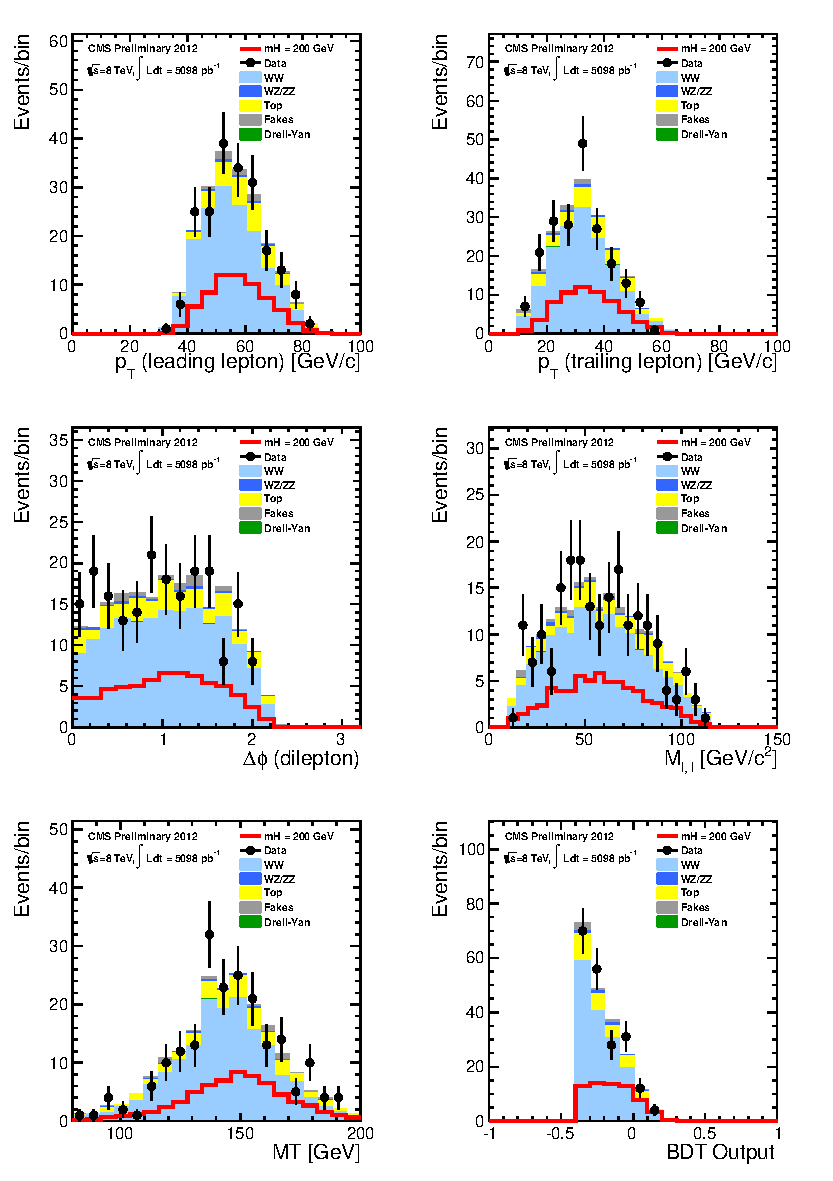
\includegraphics[width=1.0\textwidth]{figures/hww_bdthi_analysis18_200_ALL_of_0j.pdf}
\caption{Kinematic distributions in the 0-jet bin in the opposite flavor final states for $m_{H}=200 ~\GeV$ (BDT$> -0.4$).}
\label{fig:hww_bdthi_kinematics_200_0j}
\end{figure}
\begin{figure}[!htp]
\centering
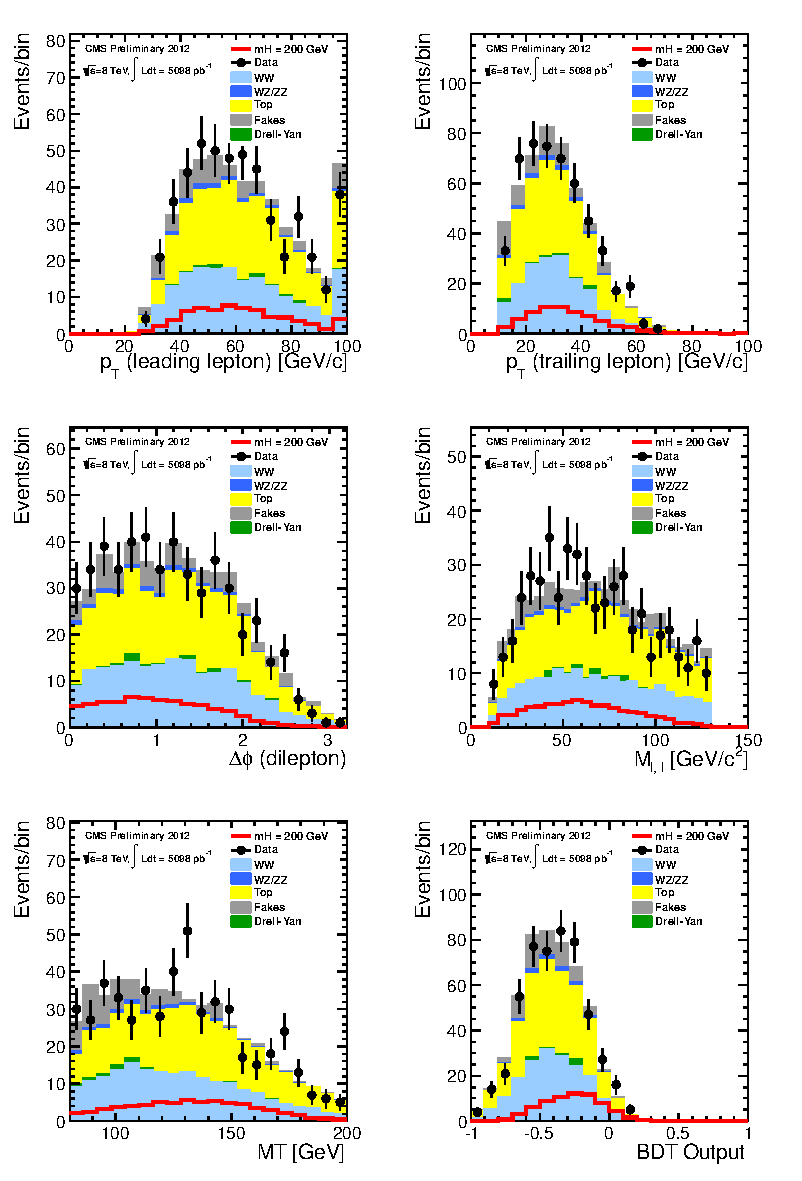
\includegraphics[width=1.0\textwidth]{figures/hww_analysis18_200_ALL_of_1j.pdf}
\caption{Kinematic distributions in the 1-jet bin in the opposite flavor final states for $m_{H}=200 ~\GeV$.}
\label{fig:hww_kinematics_200_1j}
\end{figure}
\begin{figure}[!htp]
\centering
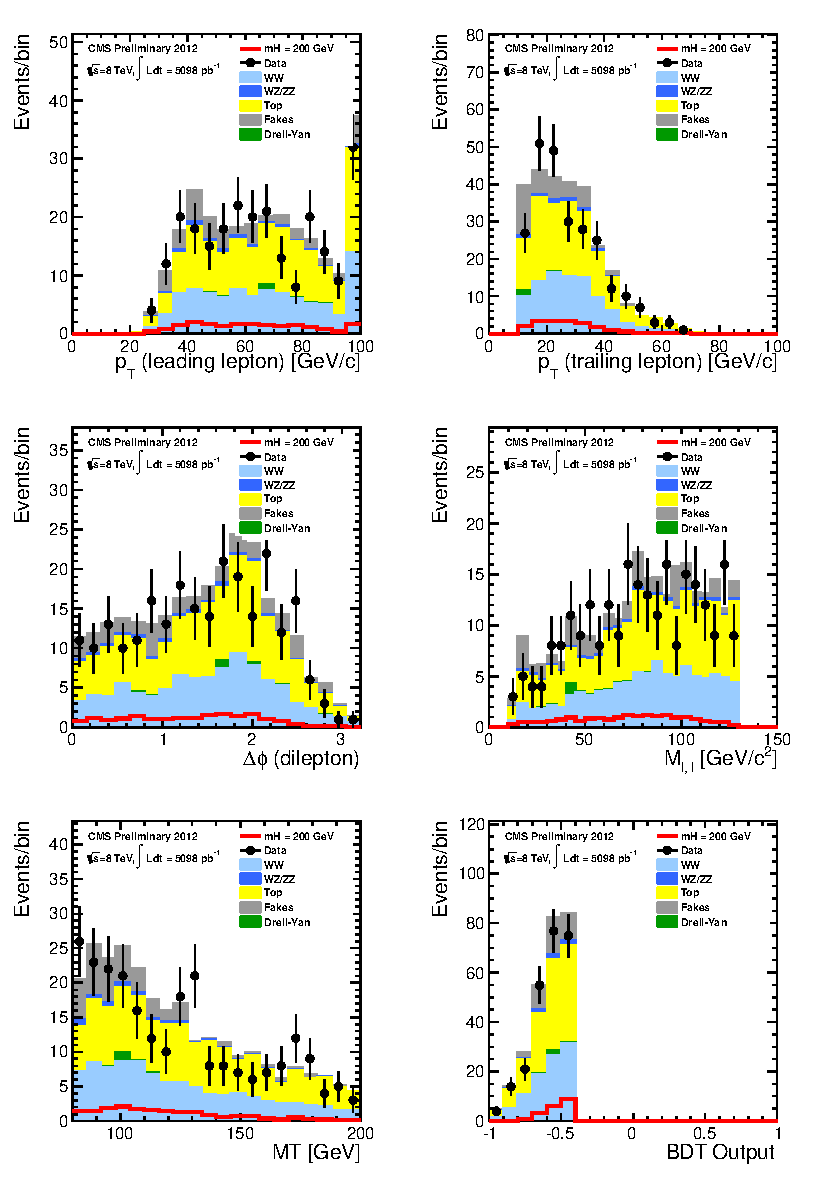
\includegraphics[width=1.0\textwidth]{figures/hww_bdtlo_analysis18_200_ALL_of_1j.pdf}
\caption{Kinematic distributions in the 1-jet bin in the opposite flavor final states for $m_{H}=200 ~\GeV$ (BDT$< -0.4$).}
\label{fig:hww_bdtlo_kinematics_200_1j}
\end{figure}
\begin{figure}[!htp]
\centering
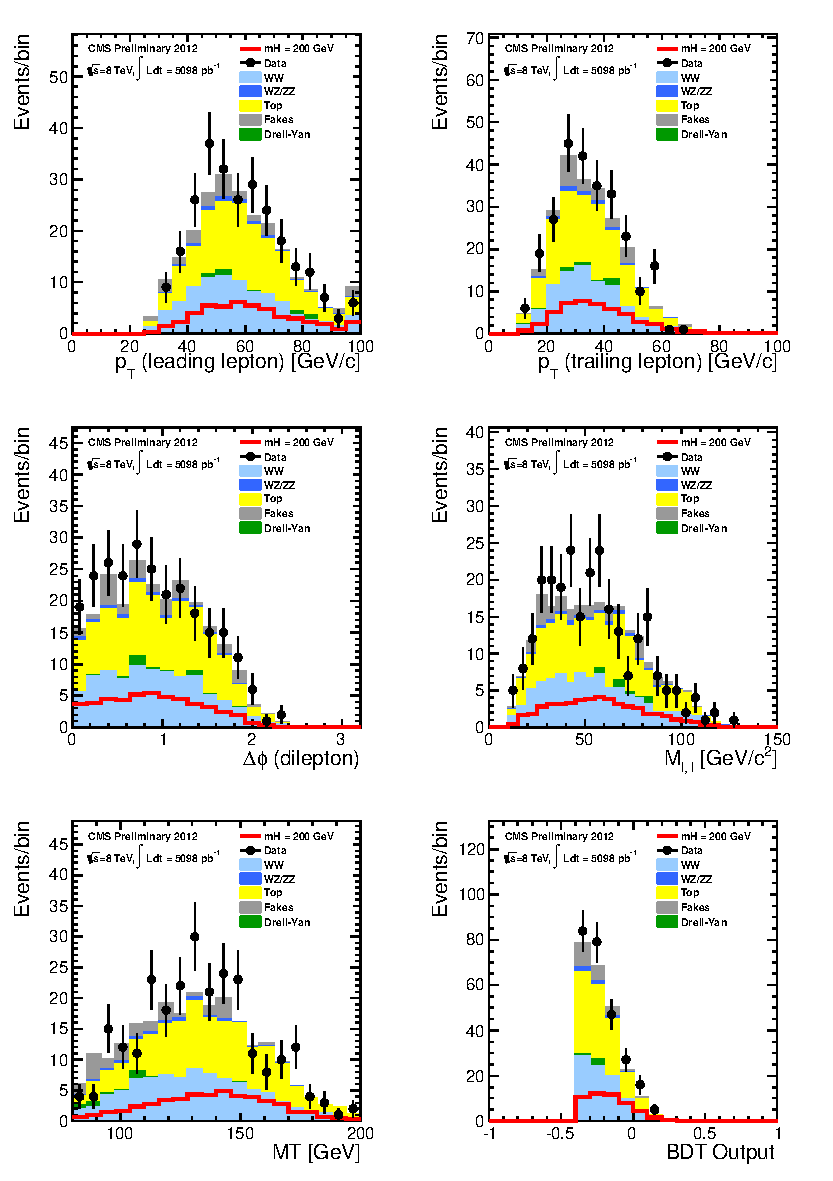
\includegraphics[width=1.0\textwidth]{figures/hww_bdthi_analysis18_200_ALL_of_1j.pdf}
\caption{Kinematic distributions in the 1-jet bin in the opposite flavor final states for $m_{H}=200 ~\GeV$ (BDT$> -0.4$).}
\label{fig:hww_bdthi_kinematics_200_1j}
\end{figure}
%%%%%%%%%%%%%%
\clearpage

\subsubsection{Tabulated yields at low BDT output}

The yields for events at low BDT output (BDT$<0.4$) are shown 
in tables \ref{tab:yields_bdtlo_0j} and \ref{tab:yields_bdtlo_1j}

\begin{table}
{%\footnotesize
 \tiny
 \begin{center}
 \begin{tabular}{l | c c | c c c c c c c c  | c c}
 \hline
 process & qqH & ggH & qqWW & ggWW & VV & Top & Zjets & Wjets & Wgamma & Ztt & $\sum$Bkg & Data \\
 \hline
110 & $0.0\pm0.0$ & $0.8\pm0.2$ & $85.0\pm9.3$ & $4.5\pm1.4$ & $2.5\pm0.2$ & $9.8\pm2.0$ & $0.3\pm0.1$ & $17.0\pm6.1$ & $1.7\pm0.5$ & $0.0\pm0.0$ & $120.9\pm11.4$ & 128 \\
115 & $0.1\pm0.0$ & $2.4\pm0.5$ & $108.3\pm11.8$ & $5.7\pm1.8$ & $3.0\pm0.2$ & $11.5\pm2.4$ & $0.4\pm0.1$ & $20.7\pm7.5$ & $1.7\pm0.5$ & $0.0\pm0.0$ & $151.2\pm14.3$ & 156 \\
120 & $0.1\pm0.0$ & $5.1\pm1.1$ & $116.5\pm12.7$ & $6.7\pm2.1$ & $3.1\pm0.2$ & $11.5\pm2.4$ & $0.4\pm0.1$ & $20.8\pm7.5$ & $1.6\pm0.5$ & $0.0\pm0.0$ & $160.6\pm15.1$ & 163 \\
125 & $0.2\pm0.0$ & $8.9\pm1.9$ & $154.5\pm16.9$ & $8.5\pm2.7$ & $4.0\pm0.3$ & $14.2\pm3.0$ & $0.7\pm0.2$ & $28.0\pm10.1$ & $1.2\pm0.4$ & $0.0\pm0.0$ & $211.1\pm20.1$ & 219 \\
130 & $0.2\pm0.0$ & $10.8\pm2.2$ & $146.4\pm16.0$ & $8.9\pm2.8$ & $3.7\pm0.3$ & $13.6\pm2.8$ & $0.7\pm0.2$ & $23.0\pm8.3$ & $0.8\pm0.2$ & $0.0\pm0.0$ & $197.1\pm18.4$ & 206 \\
135 & $0.3\pm0.0$ & $17.1\pm3.5$ & $199.4\pm21.8$ & $11.6\pm3.6$ & $4.8\pm0.4$ & $19.9\pm4.1$ & $0.8\pm0.2$ & $30.8\pm11.1$ & $2.3\pm0.7$ & $0.0\pm0.0$ & $269.5\pm25.1$ & 291 \\
140 & $0.3\pm0.0$ & $18.3\pm3.8$ & $184.4\pm20.1$ & $10.6\pm3.3$ & $4.3\pm0.3$ & $20.9\pm4.3$ & $0.7\pm0.2$ & $28.2\pm10.2$ & $1.9\pm0.6$ & $0.0\pm0.0$ & $251.0\pm23.2$ & 257 \\
145 & $0.4\pm0.0$ & $23.1\pm4.7$ & $208.7\pm22.6$ & $11.7\pm3.7$ & $5.2\pm0.4$ & $28.3\pm5.9$ & $0.8\pm0.2$ & $30.3\pm10.9$ & $2.3\pm0.7$ & $0.0\pm0.0$ & $287.1\pm26.1$ & 307 \\
150 & $0.5\pm0.0$ & $29.0\pm6.1$ & $211.5\pm22.9$ & $12.0\pm3.8$ & $5.2\pm0.4$ & $30.0\pm6.2$ & $0.8\pm0.2$ & $33.8\pm12.2$ & $2.3\pm0.7$ & $0.0\pm0.0$ & $295.5\pm27.0$ & 313 \\
160 & $0.5\pm0.0$ & $32.4\pm6.8$ & $230.1\pm25.0$ & $14.2\pm4.4$ & $5.8\pm0.4$ & $36.0\pm7.5$ & $0.8\pm0.3$ & $38.4\pm13.8$ & $3.8\pm1.2$ & $0.0\pm0.0$ & $329.2\pm29.9$ & 355 \\
170 & $0.7\pm0.1$ & $34.2\pm7.3$ & $226.8\pm24.6$ & $13.6\pm4.2$ & $5.9\pm0.4$ & $36.2\pm7.5$ & $0.8\pm0.2$ & $43.6\pm15.7$ & $5.1\pm1.6$ & $0.0\pm0.0$ & $331.9\pm30.5$ & 362 \\
180 & $1.2\pm0.1$ & $60.8\pm13.0$ & $315.1\pm34.6$ & $17.7\pm5.5$ & $8.0\pm0.6$ & $43.2\pm9.0$ & $0.9\pm0.3$ & $59.4\pm21.4$ & $9.1\pm2.8$ & $0.0\pm0.0$ & $453.4\pm42.2$ & 498 \\
190 & $0.9\pm0.1$ & $41.5\pm9.1$ & $318.1\pm35.7$ & $16.7\pm5.3$ & $8.2\pm0.6$ & $41.3\pm8.6$ & $0.9\pm0.3$ & $58.3\pm21.0$ & $9.9\pm3.0$ & $0.0\pm0.0$ & $453.3\pm42.7$ & 512 \\
200 & $1.1\pm0.1$ & $53.4\pm11.7$ & $411.3\pm47.1$ & $23.4\pm7.4$ & $10.3\pm0.8$ & $55.3\pm11.5$ & $1.0\pm0.3$ & $68.2\pm24.6$ & $10.9\pm3.3$ & $0.0\pm0.0$ & $580.3\pm55.0$ & 660 \\
250 & $0.9\pm0.1$ & $37.3\pm8.8$ & $505.5\pm50.4$ & $31.7\pm9.7$ & $13.9\pm1.1$ & $88.6\pm18.4$ & $1.9\pm0.8$ & $78.7\pm28.3$ & $12.4\pm3.8$ & $0.0\pm0.0$ & $732.6\pm61.6$ & 901 \\
300 & $0.6\pm0.0$ & $21.0\pm5.4$ & $520.1\pm51.9$ & $34.6\pm10.6$ & $14.4\pm1.1$ & $91.0\pm18.9$ & $2.0\pm0.9$ & $78.6\pm28.3$ & $13.2\pm4.1$ & $0.0\pm0.0$ & $753.9\pm63.1$ & 916 \\
350 & $0.4\pm0.0$ & $16.7\pm4.8$ & $536.7\pm53.5$ & $35.9\pm11.0$ & $14.9\pm1.1$ & $93.7\pm19.5$ & $2.1\pm0.9$ & $77.7\pm28.0$ & $13.0\pm4.0$ & $0.0\pm0.0$ & $774.0\pm64.6$ & 959 \\
400 & $0.2\pm0.0$ & $9.0\pm2.6$ & $529.1\pm52.8$ & $35.3\pm10.8$ & $14.7\pm1.1$ & $91.4\pm19.0$ & $2.1\pm0.9$ & $77.4\pm27.9$ & $13.2\pm4.1$ & $0.0\pm0.0$ & $763.2\pm63.7$ & 956 \\
450 & $0.2\pm0.0$ & $6.0\pm1.9$ & $558.3\pm55.7$ & $37.0\pm11.4$ & $15.6\pm1.2$ & $100.6\pm20.9$ & $2.1\pm0.9$ & $81.4\pm29.3$ & $13.0\pm4.0$ & $0.0\pm0.0$ & $808.1\pm67.4$ & 1006 \\
500 & $0.1\pm0.0$ & $3.4\pm1.2$ & $566.9\pm56.5$ & $37.6\pm11.5$ & $16.0\pm1.2$ & $104.9\pm21.8$ & $2.1\pm0.9$ & $82.4\pm29.7$ & $13.0\pm4.0$ & $0.0\pm0.0$ & $822.9\pm68.6$ & 1018 \\
550 & $0.1\pm0.0$ & $2.1\pm0.9$ & $571.3\pm57.0$ & $38.1\pm11.7$ & $16.0\pm1.2$ & $107.5\pm22.4$ & $2.1\pm0.9$ & $82.6\pm29.7$ & $13.0\pm4.0$ & $0.0\pm0.0$ & $830.5\pm69.2$ & 1038 \\
600 & $0.1\pm0.0$ & $1.0\pm0.5$ & $567.7\pm56.6$ & $37.8\pm11.6$ & $16.0\pm1.2$ & $106.6\pm22.2$ & $2.1\pm0.9$ & $82.4\pm29.7$ & $13.0\pm4.0$ & $0.0\pm0.0$ & $825.6\pm68.8$ & 1025 \\
\hline
\end{tabular}
\end{center}
\label{tab:yields_bdtlo_0j}
\caption{Yields for BDT output $<0.4$ in opposite flavor events with zero jets. The uncertainties are statistical and systematic.}}
\end{table}

\begin{table}
{%\footnotesize
 \tiny
 \begin{center}
 \begin{tabular}{l | c c | c c c c c c c c  | c c}
 \hline
 process & qqH & ggH & qqWW & ggWW & VV & Top & Zjets & Wjets & Wgamma & Ztt & $\sum$Bkg & Data \\
 \hline
110 & $0.0\pm0.0$ & $0.1\pm0.0$ & $14.1\pm2.6$ & $0.8\pm0.3$ & $1.3\pm0.1$ & $15.2\pm0.8$ & $2.1\pm1.0$ & $6.0\pm2.1$ & $0.4\pm0.1$ & $0.0\pm0.0$ & $39.9\pm3.6$ & 43 \\
115 & $0.1\pm0.0$ & $0.8\pm0.3$ & $23.6\pm4.4$ & $1.3\pm0.5$ & $2.2\pm0.2$ & $24.5\pm1.2$ & $2.2\pm1.0$ & $9.7\pm3.5$ & $0.4\pm0.1$ & $0.0\pm0.0$ & $63.9\pm5.9$ & 67 \\
120 & $0.2\pm0.0$ & $1.4\pm0.4$ & $23.4\pm4.4$ & $1.4\pm0.5$ & $2.2\pm0.2$ & $27.6\pm1.4$ & $2.2\pm1.0$ & $9.4\pm3.4$ & $0.4\pm0.1$ & $0.0\pm0.0$ & $66.6\pm5.8$ & 77 \\
125 & $0.4\pm0.0$ & $2.6\pm0.8$ & $32.4\pm6.1$ & $1.7\pm0.6$ & $3.0\pm0.2$ & $41.9\pm2.1$ & $2.7\pm1.1$ & $13.4\pm4.8$ & $1.2\pm0.4$ & $0.0\pm0.0$ & $96.2\pm8.1$ & 102 \\
130 & $0.1\pm0.0$ & $0.7\pm0.2$ & $17.6\pm3.3$ & $0.9\pm0.3$ & $1.4\pm0.1$ & $24.6\pm1.2$ & $0.8\pm0.5$ & $6.1\pm2.2$ & $1.0\pm0.3$ & $0.0\pm0.0$ & $52.4\pm4.2$ & 47 \\
135 & $0.9\pm0.1$ & $6.3\pm2.0$ & $46.0\pm8.6$ & $2.2\pm0.8$ & $3.8\pm0.3$ & $58.9\pm2.9$ & $3.2\pm1.3$ & $16.6\pm6.0$ & $1.5\pm0.5$ & $0.0\pm0.0$ & $132.3\pm11.0$ & 144 \\
140 & $0.2\pm0.0$ & $1.6\pm0.5$ & $27.0\pm5.1$ & $1.4\pm0.5$ & $2.0\pm0.2$ & $36.4\pm1.8$ & $1.3\pm1.0$ & $10.0\pm3.6$ & $1.1\pm0.4$ & $0.0\pm0.0$ & $79.3\pm6.6$ & 80 \\
145 & $0.5\pm0.0$ & $2.4\pm0.7$ & $37.7\pm7.5$ & $1.8\pm0.6$ & $2.8\pm0.2$ & $51.7\pm2.6$ & $1.3\pm1.0$ & $16.1\pm5.8$ & $1.6\pm0.5$ & $0.0\pm0.0$ & $113.1\pm9.9$ & 102 \\
150 & $0.4\pm0.0$ & $2.7\pm0.8$ & $37.6\pm7.4$ & $1.9\pm0.7$ & $2.7\pm0.2$ & $53.8\pm2.7$ & $0.4\pm0.2$ & $14.4\pm5.2$ & $1.8\pm0.5$ & $0.0\pm0.0$ & $112.5\pm9.5$ & 109 \\
160 & $0.5\pm0.0$ & $2.8\pm0.9$ & $42.1\pm8.3$ & $2.2\pm0.8$ & $3.0\pm0.2$ & $60.3\pm3.0$ & $1.8\pm0.9$ & $17.1\pm6.1$ & $1.8\pm0.5$ & $0.0\pm0.0$ & $128.2\pm10.9$ & 124 \\
170 & $0.6\pm0.0$ & $2.7\pm0.8$ & $34.0\pm6.7$ & $1.3\pm0.5$ & $2.2\pm0.2$ & $51.1\pm2.6$ & $1.4\pm0.8$ & $14.2\pm5.1$ & $1.7\pm0.5$ & $0.0\pm0.0$ & $106.1\pm8.9$ & 100 \\
180 & $2.6\pm0.2$ & $15.8\pm4.8$ & $75.2\pm13.8$ & $3.3\pm1.1$ & $4.9\pm0.4$ & $98.9\pm4.9$ & $3.3\pm1.4$ & $27.0\pm9.7$ & $2.9\pm0.9$ & $0.0\pm0.0$ & $215.5\pm17.7$ & 206 \\
190 & $0.3\pm0.0$ & $1.8\pm0.5$ & $25.2\pm5.0$ & $1.1\pm0.4$ & $1.5\pm0.1$ & $39.6\pm2.0$ & $0.1\pm0.0$ & $8.6\pm3.1$ & $0.2\pm0.1$ & $0.0\pm0.0$ & $76.3\pm6.2$ & 68 \\
200 & $2.7\pm0.2$ & $15.9\pm4.7$ & $89.9\pm19.0$ & $4.2\pm1.5$ & $6.4\pm0.5$ & $125.0\pm6.2$ & $2.1\pm1.1$ & $36.0\pm12.9$ & $3.0\pm0.9$ & $0.0\pm0.0$ & $266.7\pm24.0$ & 246 \\
250 & $2.8\pm0.2$ & $17.2\pm5.1$ & $166.3\pm24.0$ & $10.0\pm3.1$ & $13.0\pm1.0$ & $222.4\pm11.1$ & $5.6\pm1.9$ & $53.3\pm19.2$ & $7.5\pm2.3$ & $0.0\pm0.0$ & $477.9\pm33.0$ & 483 \\
300 & $1.6\pm0.1$ & $10.0\pm3.0$ & $166.6\pm24.1$ & $10.3\pm3.2$ & $13.2\pm1.0$ & $225.7\pm11.3$ & $5.6\pm1.9$ & $54.8\pm19.7$ & $8.4\pm2.6$ & $0.0\pm0.0$ & $484.5\pm33.4$ & 518 \\
350 & $1.0\pm0.1$ & $7.8\pm2.4$ & $177.2\pm25.6$ & $10.8\pm3.3$ & $13.4\pm1.0$ & $239.1\pm12.0$ & $5.6\pm1.9$ & $55.7\pm20.1$ & $9.4\pm2.9$ & $0.0\pm0.0$ & $511.2\pm35.0$ & 521 \\
400 & $0.3\pm0.0$ & $2.0\pm0.6$ & $141.0\pm20.4$ & $9.2\pm2.8$ & $11.0\pm0.8$ & $191.4\pm9.6$ & $5.6\pm1.9$ & $44.4\pm16.0$ & $8.7\pm2.7$ & $0.0\pm0.0$ & $411.3\pm27.9$ & 433 \\
450 & $0.4\pm0.1$ & $3.1\pm1.0$ & $192.8\pm27.9$ & $11.4\pm3.5$ & $14.3\pm1.1$ & $262.8\pm13.1$ & $5.7\pm1.9$ & $58.3\pm21.0$ & $9.4\pm2.9$ & $0.0\pm0.0$ & $554.7\pm37.6$ & 576 \\
500 & $0.3\pm0.1$ & $1.7\pm0.6$ & $197.4\pm28.5$ & $11.7\pm3.6$ & $14.6\pm1.1$ & $270.9\pm13.5$ & $5.7\pm1.9$ & $58.8\pm21.2$ & $9.4\pm2.9$ & $0.0\pm0.0$ & $568.5\pm38.4$ & 585 \\
550 & $0.3\pm0.1$ & $1.1\pm0.4$ & $202.0\pm29.2$ & $11.9\pm3.7$ & $14.9\pm1.1$ & $280.0\pm14.0$ & $5.7\pm1.9$ & $59.0\pm21.2$ & $9.4\pm2.9$ & $0.0\pm0.0$ & $583.0\pm39.1$ & 603 \\
600 & $0.2\pm0.1$ & $0.4\pm0.2$ & $179.7\pm26.0$ & $11.2\pm3.4$ & $13.5\pm1.0$ & $250.3\pm12.5$ & $5.7\pm1.9$ & $55.2\pm19.9$ & $9.2\pm2.8$ & $0.0\pm0.0$ & $524.7\pm35.3$ & 544 \\
\hline
\end{tabular}
\end{center}
\label{tab:yields_bdtlo_1j}
\caption{Yields for BDT output $<0.4$ in opposite flavor events with one jet. The uncertainties are statistical and systematic.}}
\end{table}

%
%
%
\clearpage
\subsubsection{Tabulated yields at high BDT output}

The yields for events at high BDT output (BDT$>=0.4$) are shown
in tables \ref{tab:yields_bdthi_0j} and \ref{tab:yields_bdthi_1j}

\begin{table}
{%\footnotesize
 \tiny
 \begin{center}
 \begin{tabular}{l | c c | c c c c c c c c  | c c}
 \hline
 process & qqH & ggH & qqWW & ggWW & VV & Top & Zjets & Wjets & Wgamma & Ztt & $\sum$Bkg & Data \\
 \hline
110 & $0.0\pm0.0$ & $2.8\pm0.6$ & $23.6\pm2.6$ & $1.7\pm0.5$ & $0.7\pm0.1$ & $1.8\pm0.4$ & $0.0\pm0.0$ & $12.1\pm4.4$ & $4.8\pm1.5$ & $0.0\pm0.0$ & $44.7\pm5.3$ & 60 \\
115 & $0.1\pm0.0$ & $5.9\pm1.2$ & $28.0\pm3.1$ & $2.0\pm0.6$ & $0.8\pm0.1$ & $2.1\pm0.4$ & $0.1\pm0.0$ & $12.6\pm4.5$ & $5.0\pm1.5$ & $0.0\pm0.0$ & $50.5\pm5.7$ & 70 \\
120 & $0.1\pm0.0$ & $11.7\pm2.5$ & $45.7\pm5.0$ & $2.7\pm0.8$ & $1.3\pm0.1$ & $4.5\pm0.9$ & $0.1\pm0.0$ & $16.5\pm5.9$ & $5.5\pm1.7$ & $0.0\pm0.0$ & $76.2\pm8.0$ & 103 \\
125 & $0.3\pm0.0$ & $22.1\pm4.6$ & $63.9\pm7.0$ & $3.8\pm1.2$ & $1.8\pm0.1$ & $6.3\pm1.3$ & $0.1\pm0.0$ & $18.5\pm6.6$ & $6.1\pm1.9$ & $0.0\pm0.0$ & $100.3\pm10.0$ & 132 \\
130 & $0.5\pm0.0$ & $37.7\pm7.8$ & $99.5\pm10.9$ & $5.9\pm1.9$ & $2.6\pm0.2$ & $9.0\pm1.9$ & $0.2\pm0.0$ & $25.8\pm9.3$ & $6.5\pm2.0$ & $0.0\pm0.0$ & $149.5\pm14.7$ & 176 \\
135 & $0.8\pm0.1$ & $52.8\pm10.8$ & $109.2\pm11.9$ & $6.8\pm2.1$ & $2.7\pm0.2$ & $10.2\pm2.1$ & $0.2\pm0.0$ & $25.1\pm9.0$ & $6.5\pm2.0$ & $0.0\pm0.0$ & $160.6\pm15.4$ & 182 \\
140 & $1.2\pm0.1$ & $75.7\pm15.5$ & $148.5\pm16.2$ & $9.9\pm3.1$ & $3.6\pm0.3$ & $13.5\pm2.8$ & $0.2\pm0.0$ & $29.0\pm10.5$ & $7.0\pm2.1$ & $0.0\pm0.0$ & $211.7\pm19.9$ & 247 \\
145 & $1.4\pm0.1$ & $98.0\pm20.1$ & $157.4\pm17.1$ & $11.1\pm3.5$ & $4.0\pm0.3$ & $15.5\pm3.2$ & $0.3\pm0.0$ & $29.4\pm10.6$ & $6.8\pm2.1$ & $0.0\pm0.0$ & $224.4\pm20.7$ & 271 \\
150 & $1.8\pm0.1$ & $123.9\pm26.0$ & $174.2\pm18.9$ & $12.9\pm4.0$ & $4.4\pm0.3$ & $16.9\pm3.5$ & $0.2\pm0.0$ & $27.0\pm9.7$ & $6.8\pm2.1$ & $0.0\pm0.0$ & $242.4\pm22.0$ & 289 \\
160 & $3.2\pm0.2$ & $191.3\pm40.1$ & $182.8\pm19.8$ & $14.2\pm4.4$ & $4.3\pm0.3$ & $17.9\pm3.7$ & $0.2\pm0.0$ & $24.0\pm8.6$ & $6.0\pm1.9$ & $0.0\pm0.0$ & $249.4\pm22.5$ & 286 \\
170 & $3.5\pm0.3$ & $184.3\pm39.5$ & $202.4\pm22.0$ & $17.2\pm5.4$ & $4.6\pm0.3$ & $22.7\pm4.7$ & $0.3\pm0.0$ & $21.1\pm7.6$ & $5.2\pm1.6$ & $0.0\pm0.0$ & $273.4\pm24.4$ & 308 \\
180 & $2.7\pm0.2$ & $127.7\pm27.4$ & $166.1\pm18.3$ & $16.7\pm5.2$ & $3.6\pm0.3$ & $23.6\pm4.9$ & $0.2\pm0.0$ & $8.8\pm3.2$ & $1.7\pm0.5$ & $0.0\pm0.0$ & $220.7\pm19.9$ & 251 \\
190 & $2.1\pm0.2$ & $95.5\pm20.9$ & $198.2\pm22.2$ & $20.0\pm6.3$ & $4.3\pm0.3$ & $34.7\pm7.2$ & $0.3\pm0.0$ & $12.4\pm4.5$ & $1.1\pm0.3$ & $0.0\pm0.0$ & $271.2\pm24.6$ & 304 \\
200 & $1.4\pm0.1$ & $63.4\pm13.9$ & $142.9\pm16.4$ & $15.8\pm5.0$ & $3.1\pm0.2$ & $30.6\pm6.4$ & $0.2\pm0.0$ & $4.8\pm1.7$ & $0.7\pm0.2$ & $0.0\pm0.0$ & $197.9\pm18.3$ & 201 \\
250 & $0.9\pm0.1$ & $33.0\pm7.8$ & $93.3\pm9.3$ & $7.8\pm2.4$ & $2.7\pm0.2$ & $35.1\pm7.3$ & $0.3\pm0.1$ & $7.1\pm2.5$ & $0.9\pm0.3$ & $0.0\pm0.0$ & $147.1\pm12.3$ & 176 \\
300 & $0.8\pm0.1$ & $28.0\pm7.2$ & $93.3\pm9.3$ & $6.2\pm1.9$ & $2.8\pm0.2$ & $39.0\pm8.1$ & $0.1\pm0.0$ & $8.9\pm3.2$ & $0.5\pm0.2$ & $0.0\pm0.0$ & $150.8\pm12.9$ & 184 \\
350 & $0.6\pm0.1$ & $28.4\pm8.2$ & $83.4\pm8.3$ & $5.4\pm1.7$ & $2.4\pm0.2$ & $38.2\pm7.9$ & $0.1\pm0.0$ & $10.2\pm3.7$ & $1.1\pm0.3$ & $0.0\pm0.0$ & $140.8\pm12.2$ & 156 \\
400 & $0.5\pm0.1$ & $24.6\pm7.0$ & $94.8\pm9.5$ & $6.3\pm1.9$ & $2.7\pm0.2$ & $41.9\pm8.7$ & $0.1\pm0.0$ & $10.9\pm3.9$ & $0.8\pm0.3$ & $0.0\pm0.0$ & $157.5\pm13.6$ & 170 \\
450 & $0.4\pm0.1$ & $15.0\pm4.8$ & $67.7\pm6.8$ & $4.7\pm1.4$ & $1.9\pm0.1$ & $33.1\pm6.9$ & $0.1\pm0.0$ & $7.1\pm2.6$ & $1.1\pm0.3$ & $0.0\pm0.0$ & $115.6\pm10.1$ & 125 \\
500 & $0.3\pm0.1$ & $9.6\pm3.6$ & $60.3\pm6.0$ & $4.2\pm1.3$ & $1.6\pm0.1$ & $29.2\pm6.1$ & $0.0\pm0.0$ & $6.2\pm2.2$ & $1.2\pm0.4$ & $0.0\pm0.0$ & $102.7\pm8.9$ & 115 \\
550 & $0.3\pm0.1$ & $6.4\pm2.7$ & $56.9\pm5.7$ & $3.7\pm1.1$ & $1.5\pm0.1$ & $26.8\pm5.6$ & $0.0\pm0.0$ & $6.0\pm2.2$ & $1.4\pm0.4$ & $0.0\pm0.0$ & $96.4\pm8.3$ & 95 \\
600 & $0.2\pm0.1$ & $4.2\pm2.0$ & $60.7\pm6.1$ & $4.0\pm1.2$ & $1.6\pm0.1$ & $27.8\pm5.8$ & $0.0\pm0.0$ & $6.4\pm2.3$ & $1.4\pm0.4$ & $0.0\pm0.0$ & $102.0\pm8.8$ & 108 \\
\hline
\end{tabular}
\end{center}
\label{tab:yields_bdthi_0j}
\caption{Yields for BDT output $>=0.4$ in opposite flavor events with zero jets. The uncertainties are statistical and systematic.}}
\end{table}

\begin{table}
{%\footnotesize
 \tiny
 \begin{center}
 \begin{tabular}{l | c c | c c c c c c c c  | c c}
 \hline
 process & qqH & ggH & qqWW & ggWW & VV & Top & Zjets & Wjets & Wgamma & Ztt & $\sum$Bkg & Data \\
 \hline
110 & $0.2\pm0.0$ & $1.5\pm0.5$ & $13.8\pm2.6$ & $0.9\pm0.3$ & $1.7\pm0.1$ & $14.4\pm0.7$ & $1.5\pm1.1$ & $12.0\pm4.3$ & $5.5\pm1.7$ & $0.0\pm0.0$ & $49.8\pm5.5$ & 39 \\
115 & $0.3\pm0.0$ & $2.7\pm0.9$ & $9.9\pm1.9$ & $0.7\pm0.2$ & $1.3\pm0.1$ & $10.8\pm0.5$ & $1.4\pm1.1$ & $10.6\pm3.8$ & $5.5\pm1.7$ & $0.0\pm0.0$ & $40.2\pm4.7$ & 33 \\
120 & $0.7\pm0.1$ & $5.6\pm1.8$ & $15.0\pm2.8$ & $0.9\pm0.3$ & $1.9\pm0.1$ & $15.1\pm0.8$ & $1.5\pm1.1$ & $13.3\pm4.8$ & $5.6\pm1.7$ & $0.0\pm0.0$ & $53.2\pm6.0$ & 44 \\
125 & $1.3\pm0.1$ & $10.0\pm3.2$ & $19.5\pm3.6$ & $1.3\pm0.4$ & $2.4\pm0.2$ & $20.2\pm1.0$ & $1.5\pm1.1$ & $16.0\pm5.8$ & $6.0\pm1.8$ & $0.0\pm0.0$ & $66.9\pm7.2$ & 59 \\
130 & $2.5\pm0.2$ & $19.2\pm6.2$ & $40.0\pm7.5$ & $2.6\pm0.9$ & $4.3\pm0.3$ & $46.9\pm2.3$ & $3.5\pm1.5$ & $24.3\pm8.8$ & $6.3\pm1.9$ & $0.0\pm0.0$ & $128.0\pm12.1$ & 135 \\
135 & $2.7\pm0.2$ & $22.7\pm7.1$ & $28.0\pm5.3$ & $2.0\pm0.7$ & $3.2\pm0.2$ & $32.0\pm1.6$ & $2.2\pm1.2$ & $18.7\pm6.7$ & $6.0\pm1.8$ & $0.0\pm0.0$ & $92.2\pm9.0$ & 95 \\
140 & $4.8\pm0.4$ & $37.3\pm11.7$ & $52.9\pm9.9$ & $3.6\pm1.2$ & $5.4\pm0.4$ & $63.9\pm3.2$ & $4.1\pm1.6$ & $26.6\pm9.6$ & $6.3\pm1.9$ & $0.0\pm0.0$ & $162.9\pm14.4$ & 177 \\
145 & $5.8\pm0.4$ & $49.2\pm15.4$ & $61.3\pm12.1$ & $4.4\pm1.6$ & $5.8\pm0.4$ & $71.0\pm3.6$ & $4.1\pm1.6$ & $27.3\pm9.8$ & $6.3\pm1.9$ & $0.0\pm0.0$ & $180.3\pm16.3$ & 197 \\
150 & $7.6\pm0.6$ & $59.2\pm18.3$ & $67.2\pm13.3$ & $4.8\pm1.7$ & $6.2\pm0.5$ & $79.6\pm4.0$ & $5.1\pm1.8$ & $29.6\pm10.6$ & $6.2\pm1.9$ & $0.0\pm0.0$ & $198.6\pm17.8$ & 215 \\
160 & $11.9\pm0.9$ & $94.4\pm29.1$ & $73.4\pm14.5$ & $5.4\pm1.9$ & $6.4\pm0.5$ & $90.2\pm4.5$ & $3.7\pm1.6$ & $28.2\pm10.1$ & $6.2\pm1.9$ & $0.0\pm0.0$ & $213.6\pm18.5$ & 230 \\
170 & $13.2\pm1.0$ & $96.5\pm29.6$ & $89.1\pm17.6$ & $6.9\pm2.4$ & $7.6\pm0.6$ & $113.9\pm5.7$ & $4.1\pm1.7$ & $31.3\pm11.3$ & $6.3\pm1.9$ & $0.0\pm0.0$ & $259.2\pm22.0$ & 276 \\
180 & $10.4\pm0.8$ & $71.5\pm21.8$ & $76.9\pm14.1$ & $6.2\pm2.2$ & $6.0\pm0.5$ & $92.7\pm4.6$ & $2.2\pm1.2$ & $21.6\pm7.8$ & $5.9\pm1.8$ & $0.0\pm0.0$ & $211.6\pm17.0$ & 231 \\
190 & $10.0\pm0.7$ & $64.2\pm19.6$ & $139.1\pm27.5$ & $9.2\pm3.2$ & $10.2\pm0.8$ & $176.2\pm8.8$ & $5.5\pm1.9$ & $43.2\pm15.5$ & $8.6\pm2.6$ & $0.0\pm0.0$ & $392.0\pm33.1$ & 402 \\
200 & $6.2\pm0.5$ & $41.6\pm12.2$ & $82.0\pm17.4$ & $6.5\pm2.4$ & $6.0\pm0.5$ & $110.8\pm5.5$ & $3.5\pm1.5$ & $17.5\pm6.3$ & $5.9\pm1.8$ & $0.0\pm0.0$ & $232.3\pm19.6$ & 258 \\
250 & $2.8\pm0.2$ & $20.4\pm6.0$ & $62.3\pm9.0$ & $3.1\pm1.0$ & $3.2\pm0.2$ & $99.2\pm5.0$ & $0.1\pm0.0$ & $11.6\pm4.2$ & $1.6\pm0.5$ & $0.0\pm0.0$ & $181.2\pm11.1$ & 189 \\
300 & $2.7\pm0.2$ & $19.0\pm5.7$ & $71.1\pm10.3$ & $3.2\pm1.0$ & $3.6\pm0.3$ & $106.6\pm5.3$ & $0.1\pm0.0$ & $12.1\pm4.4$ & $0.6\pm0.2$ & $0.0\pm0.0$ & $197.3\pm12.4$ & 186 \\
350 & $2.3\pm0.2$ & $21.0\pm6.4$ & $64.6\pm9.3$ & $2.9\pm0.9$ & $3.5\pm0.3$ & $99.3\pm5.0$ & $0.1\pm0.0$ & $12.1\pm4.4$ & $0.4\pm0.1$ & $0.0\pm0.0$ & $182.9\pm11.5$ & 193 \\
400 & $2.0\pm0.2$ & $20.1\pm6.2$ & $103.2\pm14.9$ & $4.5\pm1.4$ & $6.1\pm0.5$ & $149.9\pm7.5$ & $0.2\pm0.0$ & $23.7\pm8.5$ & $1.2\pm0.4$ & $0.0\pm0.0$ & $288.7\pm18.8$ & 286 \\
450 & $1.3\pm0.2$ & $11.7\pm3.8$ & $53.0\pm7.7$ & $2.3\pm0.7$ & $2.8\pm0.2$ & $79.5\pm4.0$ & $0.1\pm0.0$ & $10.0\pm3.6$ & $0.5\pm0.2$ & $0.0\pm0.0$ & $148.3\pm9.4$ & 144 \\
500 & $1.0\pm0.2$ & $8.0\pm2.8$ & $49.0\pm7.1$ & $2.1\pm0.6$ & $2.6\pm0.2$ & $71.9\pm3.6$ & $0.1\pm0.0$ & $9.8\pm3.5$ & $0.5\pm0.2$ & $0.0\pm0.0$ & $136.0\pm8.7$ & 136 \\
550 & $0.8\pm0.2$ & $5.6\pm2.2$ & $44.6\pm6.4$ & $1.8\pm0.6$ & $2.2\pm0.2$ & $63.1\pm3.2$ & $0.1\pm0.0$ & $10.0\pm3.6$ & $0.5\pm0.2$ & $0.0\pm0.0$ & $122.3\pm8.0$ & 119 \\
600 & $0.7\pm0.2$ & $4.0\pm1.8$ & $67.1\pm9.7$ & $2.6\pm0.8$ & $3.7\pm0.3$ & $92.9\pm4.6$ & $0.1\pm0.0$ & $13.9\pm5.0$ & $0.8\pm0.2$ & $0.0\pm0.0$ & $180.9\pm11.9$ & 180 \\
\hline
\end{tabular}
\end{center}
\label{tab:yields_bdthi_1j}
\caption{Yields for BDT output $>=0.4$ in opposite flavor events with one jet. The uncertainties are statistical and systematic.}}
\end{table}

